\documentclass[12pt,a4paper]{report}

% ============================================================
% PACKAGES
% ============================================================
\usepackage[utf8]{inputenc}
\usepackage[T1]{fontenc}
\usepackage{mathptmx}                   % Times New Roman
\usepackage{setspace}                    % Line spacing
\usepackage[margin=1in]{geometry}        % 1-inch margins
\usepackage{graphicx}                    % Images
\usepackage{float}                       % [H] placement
\usepackage{booktabs}                    % Professional tables
\usepackage{caption}                     % Caption formatting
\usepackage{subcaption}                  % Side-by-side figures
\usepackage{amsmath,amssymb}             % Math
\usepackage{hyperref}                    % Clickable links
\usepackage[numbers]{natbib}             % Citations
\usepackage{enumitem}                    % List formatting
\usepackage{tabularx}                    % Flexible tables
\usepackage{array}                       % Table column types
\usepackage{xcolor}                      % Colours
\usepackage{fancyhdr}                    % Headers/footers
\usepackage{titlesec}                    % Section formatting
\usepackage{pdfpages}                    % Include PDFs if needed

% ============================================================
% SETTINGS
% ============================================================
\onehalfspacing
\graphicspath{{images/}}

\hypersetup{
    colorlinks=true,
    linkcolor=black,
    citecolor=blue,
    urlcolor=blue
}

\captionsetup{
    font=small,
    labelfont=bf,
    skip=8pt
}

% Page style
\pagestyle{fancy}
\fancyhf{}
\fancyhead[L]{\small\nouppercase{\leftmark}}
\fancyhead[R]{}
\fancyfoot[C]{\thepage}
\renewcommand{\headrulewidth}{0.4pt}

% Chapter title formatting
\titleformat{\chapter}[display]
{\normalfont\Large\bfseries}{\chaptertitlename\ \thechapter}{12pt}{\LARGE}
\titlespacing*{\chapter}{0pt}{-20pt}{20pt}

% ============================================================
% DOCUMENT START
% ============================================================
\begin{document}

% ============================================================
% COVER PAGE
% ============================================================
\begin{titlepage}
    \centering
    \vspace*{0.5cm}

    
\includegraphics[width=0.35\textwidth]{university_logo.png}\\[0.8cm]

    {\Large\textbf{QUEEN MARY, UNIVERSITY OF LONDON}}\\[0.3cm]
    {\large SCHOOL OF ELECTRONIC ENGINEERING AND COMPUTER SCIENCE}\\[2cm]

    {\Huge\textbf{ML-Based Parameter Optimisation\\[0.3cm]
    for Graphene Metamaterial\\[0.3cm]
    THz Modulators}}\\[2cm]

    {\Large Final Year Project Report}\\[2cm]

    {\large
    \textbf{Student:} Linah Salem Alrejaee\\[0.3cm]
    \textbf{Student ID:} 231001766\\[0.3cm]
    \textbf{Programme:} BSc Computer Science\\[0.3cm]
    \textbf{Supervisor:} Dr.\ Riccardo Degl'Innocenti\\[0.3cm]
    \textbf{Institution:} Queen Mary University of London\\[0.3cm]
    \textbf{Date:} March 2026
    }

    \vfill
\end{titlepage}

% ============================================================
% ABSTRACT
% ============================================================
\chapter*{Abstract}
\addcontentsline{toc}{chapter}{Abstract}

Terahertz (THz) metamaterial modulators based on graphene offer significant potential for next-generation communication and sensing systems, yet their design relies on computationally expensive electromagnetic simulations. A single COMSOL Multiphysics simulation of the graphene metamaterial unit cell requires approximately 12 hours, severely limiting the pace of design exploration. This project presents an automated machine learning (ML) pipeline that replaces manual simulation analysis with instant surrogate predictions, enabling rapid parameter space exploration.

A dataset of 27 COMSOL simulations was constructed across three data-collection phases, spanning six geometric and material parameters: unit cell size ($d_x$), gap width ($g_w$), capacitor width ($c_w$), graphene thickness offset ($h_{\text{graph}}$), graphene width ($w_{\text{graph}}$), and gold width ($w_{\text{au}}$). Three regression models---Random Forest (RF), Gradient Boosting (GB), and Gaussian Process (GP)---were trained and evaluated using Leave-One-Out Cross-Validation (LOO~CV), appropriate for the small dataset. The Gaussian Process model achieved the strongest frequency prediction ($R^2 = 0.68$) and also led on S12 dip depth ($R^2 = 0.08$), with Random Forest providing robust feature importance rankings. On the 13 ON/OFF pairs, RF produced the most reliable modulation-performance predictions (frequency shift $R^2 = 0.47$). Feature importance analysis revealed that capacitor width ($c_w$) dominates resonant frequency prediction (importance = 0.46), while four parameters ($d_x$, $g_w$, $c_w$, $h_{\text{graph}}$) contribute comparably to S12 dip prediction (importance 0.21--0.26 each); gold width ($w_{\text{au}}$) now shows real variance-driven influence (0.05) after the Phase~3 parameter expansion.

A key discovery was that $h_{\text{graph}} = 6$ yielded the deepest S12 dip of $-16.64$~dB, a significant improvement over earlier parameter sweeps, bringing the design to within 3.36~dB of the $-20$~dB target. An interactive Streamlit dashboard was developed for real-time parameter exploration and ML-based prediction, and Phase~3 multi-objective optimisation modules (Bayesian Optimisation via Expected Improvement, plus NSGA-II) were implemented to systematically propose promising parameter combinations for subsequent COMSOL validation.

% ============================================================
% TABLE OF CONTENTS, LIST OF FIGURES, LIST OF TABLES
% ============================================================
\tableofcontents
\listoffigures
\listoftables

% ============================================================
% CHAPTER 1: INTRODUCTION
% ============================================================
\chapter{Introduction}
\label{ch:introduction}

In this chapter, I will introduce the motivation behind this project, outline the aims and objectives that have guided the research, and describe the structure of this report.

\section{Motivation}
\label{sec:motivation}

The terahertz (THz) frequency band, spanning approximately 0.1 to 10~THz, occupies a strategically important yet historically underexploited region of the electromagnetic spectrum, situated between the microwave and infrared domains. Often referred to as the ``THz gap,'' this spectral region has attracted considerable research interest due to its potential applications in high-speed wireless communications, non-invasive biomedical imaging, security screening, and spectroscopic analysis of molecular vibrations \citep{tonouchi2007}. However, the development of efficient, compact, and tunable THz components---particularly modulators capable of dynamically controlling THz wave transmission---remains a significant engineering challenge.

Metamaterials, artificially engineered structures with sub-wavelength features, offer a promising route to address this challenge. By designing periodic unit cells with carefully chosen geometric parameters, metamaterials can exhibit electromagnetic properties not found in natural materials, including negative refractive index and frequency-selective transmission \citep{pendry1999, smith2000}. When combined with active materials whose properties can be externally tuned, metamaterials become powerful platforms for reconfigurable THz devices.

Graphene, a single atomic layer of carbon atoms arranged in a honeycomb lattice, has emerged as a particularly attractive active medium for THz metamaterial modulators \citep{novoselov2004}. Its surface conductivity can be dynamically controlled via electrostatic gating, enabling switching between high-transmission (ON) and low-transmission (OFF) states without physically altering the device geometry \citep{sensale2012, lee2012}. In our device, the ON state corresponds to a graphene surface conductivity of $\sigma = 0.3$~mS, while the OFF state corresponds to $\sigma = 1.2$~mS.

The design of such metamaterial modulators requires extensive electromagnetic simulation using finite element methods, typically performed in COMSOL Multiphysics. Each simulation of our graphene metamaterial unit cell requires approximately 12 hours on a standard workstation, making systematic exploration of the multi-dimensional parameter space impractical through simulation alone. With seven geometric parameters---unit cell size ($d_x$), gap width ($g_w$), capacitor width ($c_w$), graphene thickness offset ($h_{\text{graph}}$), graphene width ($w_{\text{graph}}$), gold width ($w_{\text{au}}$), and gold top width ($w_{\text{au,top}}$)---and two conductivity states, the combinatorial design space is vast.

This project addresses this bottleneck by developing a machine learning (ML) surrogate model pipeline that can provide instant predictions of device performance metrics---specifically the S12 transmission dip depth and resonant frequency---given a set of geometric input parameters. By training ML models on a dataset of completed COMSOL simulations, we aim to enable rapid design space exploration, identify the most influential parameters, and ultimately guide the search toward optimal device configurations approaching the target S12 dip depth of $-20$~dB.

\begin{figure}[H]
    \centering
    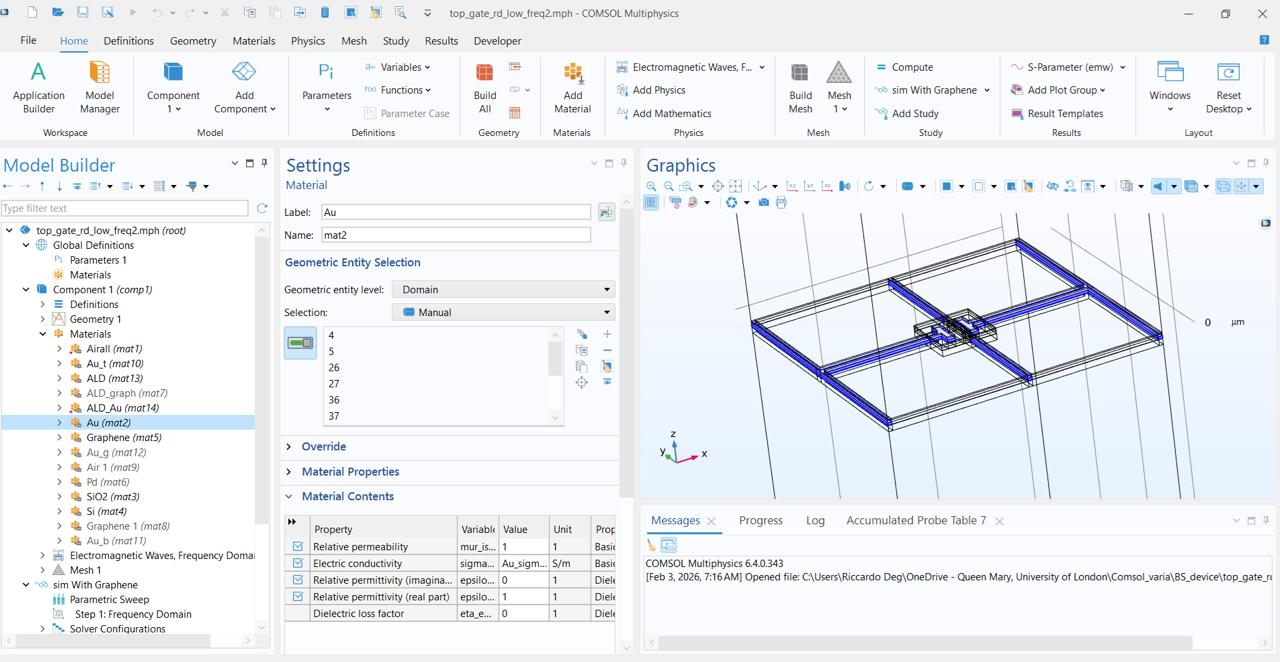
\includegraphics[width=0.75\textwidth]{comsol_3d_unit_cell.jpeg}
    \caption{3D COMSOL Multiphysics model of the graphene metamaterial unit cell, showing the layered structure including the graphene sheet, gold electrodes, and dielectric substrate.}
    \label{fig:comsol_3d}
\end{figure}

\begin{figure}[H]
    \centering
    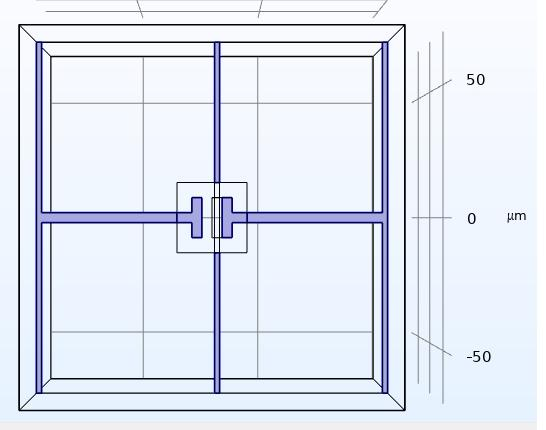
\includegraphics[width=0.75\textwidth]{comsol_topdown_unit_cell.jpeg}
    \caption{Top-down view of the unit cell showing the key geometric parameters: unit cell size ($d_x$), gap width ($g_w$), capacitor width ($c_w$), graphene width ($w_{\text{graph}}$), and gold width ($w_{\text{au}}$).}
    \label{fig:comsol_topdown}
\end{figure}

\section{Aims and Objectives}
\label{sec:aims}

The aim of this project is to develop and evaluate an automated machine learning pipeline for predicting the electromagnetic performance of graphene metamaterial THz modulators, thereby reducing the reliance on time-consuming COMSOL simulations. The specific objectives are as follows:

\begin{enumerate}[leftmargin=2cm]
    \item Parse and automate the analysis of COMSOL simulation output data, extracting geometric parameters and performance metrics from raw text files.
    \item Build and comparatively evaluate three machine learning regression models---Random Forest, Gradient Boosting, and Gaussian Process---for predicting S12 dip depth and resonant dip frequency.
    \item Apply Leave-One-Out Cross-Validation (LOO~CV) as the evaluation strategy, chosen specifically for its suitability with small datasets ($n = 27$).
    \item Conduct feature importance analysis to identify which geometric parameters most strongly influence device performance.
    \item Develop an interactive web-based dashboard using Streamlit and Plotly for real-time parameter exploration, data visualisation, and ML-based prediction.
    \item Establish a foundation for Phase~3, which will employ Bayesian Optimisation and NSGA-II multi-objective optimisation to systematically search for optimal parameter combinations.
\end{enumerate}

\section{Report Structure}
\label{sec:report_structure}

This report is structured as follows. Chapter~\ref{ch:literature} presents a critical review of the literature covering THz technology, metamaterials, graphene-based devices, and the machine learning techniques employed. Chapter~\ref{ch:design} describes the system design and implementation, including the data pipeline, ML training framework, and interactive dashboard. Chapter~\ref{ch:phase1} summarises the Phase~1 data collection and initial findings. Chapter~\ref{ch:phase2} presents the Phase~2 results, including expanded simulations, ML model evaluation, and feature importance analysis. Chapter~\ref{ch:analysis} provides an in-depth analysis and discussion of the results, including model interpretation, physical insights, and an assessment of advantages and limitations. Finally, Chapter~\ref{ch:conclusion} concludes the report with a summary of contributions and outlines future work for Phase~3.


% ============================================================
% CHAPTER 2: LITERATURE REVIEW
% ============================================================
\chapter{Literature Review}
\label{ch:literature}

In this chapter, I will review the key literature surrounding the topics of this project. This includes an overview of terahertz technology and the THz gap, the role of metamaterials and graphene in THz modulation, and a detailed examination of the machine learning techniques employed in this work. The chapter concludes by identifying the research gap that this project aims to address.

\section{Terahertz Technology and the THz Gap}
\label{sec:thz_gap}

The terahertz region of the electromagnetic spectrum, typically defined as frequencies between 0.1 and 10~THz (wavelengths of 3~mm to 30~$\mu$m), has long been recognised as one of the least developed portions of the spectrum. This ``THz gap'' exists because the frequency range falls between the operating domains of conventional electronics (which struggle above $\sim$100~GHz) and photonic devices (which are inefficient below $\sim$10~THz), creating a technological no-man's land where neither approach works efficiently \citep{tonouchi2007}.

Despite these challenges, THz radiation possesses several unique properties that make it highly attractive for applications. THz waves can penetrate many non-metallic materials (clothing, paper, plastic, ceramics) while being strongly absorbed by water, making them ideal for security screening and biomedical imaging without the ionising radiation risks of X-rays. In communications, the THz band offers enormous bandwidth potential for next-generation 6G wireless networks, with data rates potentially exceeding 100~Gbps. Spectroscopically, many molecular rotational and vibrational modes lie in the THz range, enabling fingerprint identification of chemical compounds.

The development of efficient THz modulators---devices that can dynamically control the amplitude, phase, or polarisation of THz waves---is therefore a critical enabling technology. An ideal THz modulator would exhibit a deep transmission dip (high modulation depth), operate at a tuneable frequency, switch rapidly between states, and be compact enough for integration into practical systems. Metamaterial-based approaches have emerged as one of the most promising routes to achieving these goals.

\section{Metamaterials and THz Modulators}
\label{sec:metamaterials}

Metamaterials are artificially structured materials composed of sub-wavelength unit cells, typically arranged in periodic arrays. Unlike natural materials, whose electromagnetic properties are determined by their chemical composition, the properties of metamaterials are governed by the geometry of their unit cells. This allows engineers to design materials with electromagnetic responses that do not exist in nature, such as negative refractive index, perfect absorption, and highly frequency-selective transmission \citep{pendry1999, smith2000}.

For THz modulation, metamaterials based on split-ring resonators (SRRs) and complementary structures have been widely studied. These resonant structures exhibit strong, narrowband responses characterised by transmission dips at specific frequencies determined by the geometry. The key performance metrics are:

\begin{itemize}[leftmargin=2cm]
    \item \textbf{S12 (Transmission):} The ratio of transmitted to incident power, measured in decibels (dB). A deeper negative S12 dip indicates stronger modulation. Our target is $-20$~dB.
    \item \textbf{S22 (Reflection):} The ratio of reflected to incident power. Together with S12, this characterises the complete scattering behaviour of the device.
    \item \textbf{Resonant frequency:} The frequency at which the transmission dip occurs, determined by the effective inductance and capacitance of the unit cell geometry.
\end{itemize}

The breakthrough in active THz metamaterials came with the integration of materials whose properties could be externally controlled. \citet{chen2006} demonstrated the first electrically active THz metamaterial device by incorporating semiconductor elements into the SRR gaps, enabling modulation of the resonant response through carrier injection. This established the paradigm of combining metamaterial geometry with active materials for dynamic THz control.

For our device, the modulation mechanism relies on switching between two graphene conductivity states. In the ON state ($\sigma = 0.3$~mS), the graphene is relatively transparent, allowing THz radiation to interact primarily with the metallic metamaterial structure. In the OFF state ($\sigma = 1.2$~mS), the increased graphene conductivity alters the effective impedance of the unit cell, shifting the resonant frequency and changing the dip depth. The difference between these states---quantified as frequency shift and average dip depth change---determines the modulation performance.

\section{Graphene in THz Devices}
\label{sec:graphene}

Graphene, first isolated experimentally by \citet{novoselov2004}, is a two-dimensional material consisting of a single layer of carbon atoms in a hexagonal lattice. Its exceptional electronic, optical, and mechanical properties have made it a transformative material across multiple fields of science and engineering.

For THz applications, graphene's most relevant property is its tuneable surface conductivity. The optical conductivity of graphene can be described by the Kubo formula, which accounts for both intraband and interband contributions. At THz frequencies, the intraband Drude-like contribution dominates, and the conductivity depends directly on the Fermi energy, which can be controlled through electrostatic gating or chemical doping. This means that by applying a gate voltage, one can continuously tune the graphene conductivity and thereby modulate the THz response of a metamaterial incorporating graphene.

\citet{sensale2012} demonstrated broadband graphene THz modulators exploiting intraband transitions, achieving modulation depths of up to 15\% over a broad frequency range. \citet{lee2012} reported switching THz waves using gate-controlled active graphene metamaterials, demonstrating the feasibility of integrating graphene with resonant metamaterial structures for enhanced modulation.

In our device, the graphene sheet is incorporated within the unit cell geometry and is characterised by seven parameters:
\begin{itemize}[leftmargin=2cm]
    \item $d_x$: Unit cell size (periodicity), varied across 23, 25, 27, 31, 33, and 35~$\mu$m
    \item $g_w$: Gap width between electrodes, varied across 3 and 5~$\mu$m
    \item $c_w$: Capacitor width, varied across 12, 20, and 28~$\mu$m
    \item $h_{\text{graph}}$: Graphene thickness offset, varied across $-6$, 0, 2, and 6~$\mu$m
    \item $w_{\text{graph}}$: Graphene width, fixed at 1~$\mu$m in current data
    \item $w_{\text{au}}$: Gold electrode width, fixed at 4~$\mu$m in current data
    \item $w_{\text{au,top}}$: Gold top width, fixed at 1.5~$\mu$m in current data
\end{itemize}

The challenge lies in understanding how these parameters interact to determine the S12 dip depth and resonant frequency, and in finding parameter combinations that maximise modulation performance.

\section{Machine Learning for Electromagnetic Simulation}
\label{sec:ml_em}

The application of machine learning as a surrogate for computationally expensive electromagnetic simulations has gained significant traction in recent years. Traditional electromagnetic design relies on iterative simulation: an engineer proposes a geometry, runs a simulation (which may take hours), evaluates the results, and adjusts the geometry---a process that is fundamentally limited by simulation time.

\citet{koziel2013} demonstrated the use of surrogate-assisted optimisation for microwave structures, showing that ML models trained on a small number of simulations could guide the design process more efficiently than brute-force simulation sweeps. \citet{zhang2019} applied machine learning specifically to metamaterial design, using neural networks to predict electromagnetic responses from geometric parameters and achieving significant speedups over full-wave simulation. \citet{ma2018} demonstrated deep-learning-enabled on-demand design of chiral metamaterials, showing that well-trained models could not only predict performance from geometry but also solve the inverse problem of finding geometries that produce desired responses.

For our project, the dataset size ($n = 27$) precludes the use of deep learning approaches, which typically require hundreds or thousands of training samples. Instead, we employ three classical regression models well-suited to small datasets: Random Forest, Gradient Boosting, and Gaussian Process regression. Each offers distinct advantages, as described in the following sections.

\section{Random Forest Regression}
\label{sec:rf}

Random Forest (RF) is an ensemble learning method that constructs multiple decision trees during training and outputs the average of their individual predictions \citep{breiman2001}. The key innovation is the combination of two randomisation techniques: \textit{bagging} (bootstrap aggregating), where each tree is trained on a random subsample of the data drawn with replacement, and \textit{random feature selection}, where each split in a tree considers only a random subset of features.

\begin{figure}[H]
    \centering
    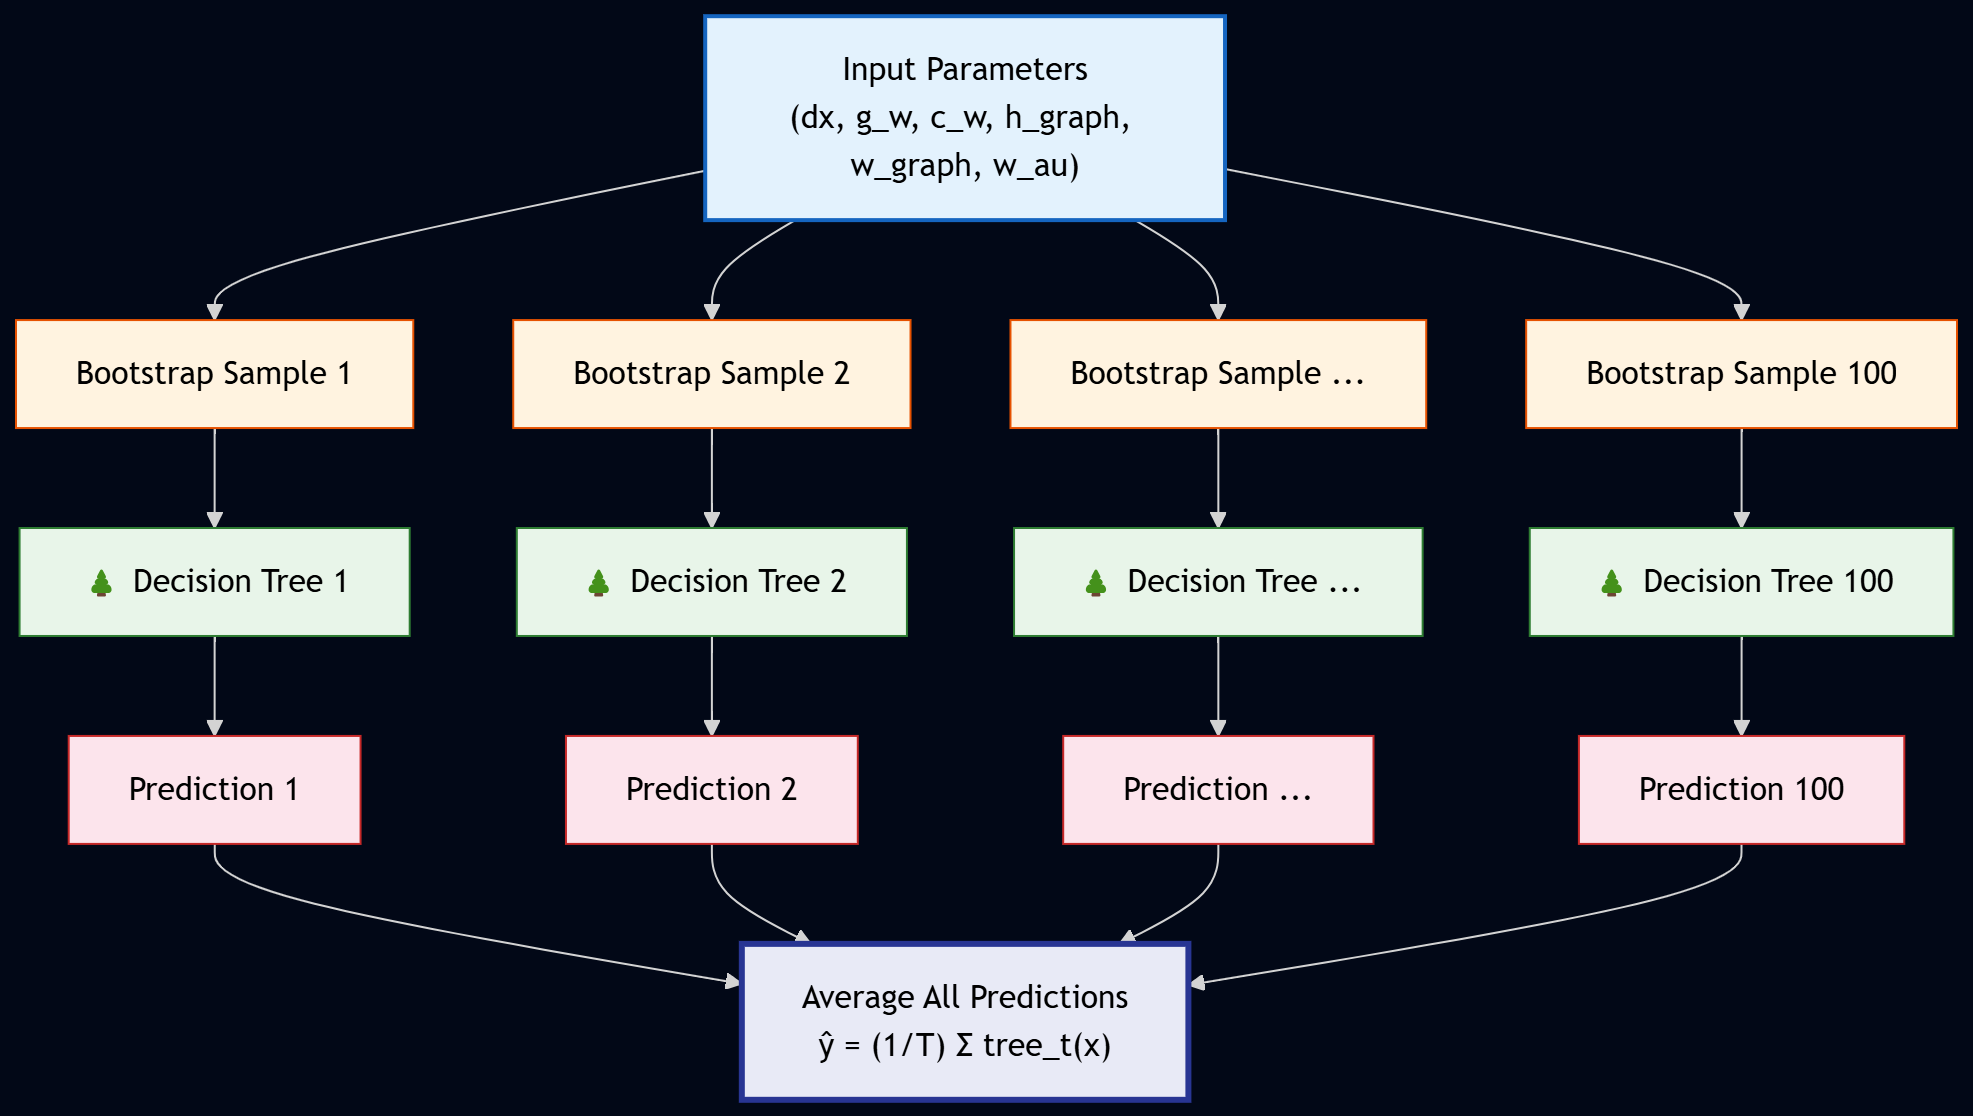
\includegraphics[width=0.85\textwidth]{mermaid_random_forest_concept.png}
    \caption{Conceptual diagram of the Random Forest algorithm. Input parameters are passed to multiple bootstrap samples, each training an independent decision tree. The final prediction is the average across all trees: $\hat{y} = \frac{1}{T}\sum_{t=1}^{T} \text{tree}_t(\mathbf{x})$.}
    \label{fig:rf_concept}
\end{figure}

The mathematical formulation for a Random Forest with $T$ trees is:

\begin{equation}
    \hat{y}(\mathbf{x}) = \frac{1}{T} \sum_{t=1}^{T} h_t(\mathbf{x})
    \label{eq:rf}
\end{equation}

\noindent where $h_t(\mathbf{x})$ is the prediction of the $t$-th decision tree for input $\mathbf{x}$.

The principal advantages of Random Forest for our application are its robustness to overfitting (through averaging over many trees), its ability to handle non-linear relationships without explicit feature engineering, and its built-in feature importance measure. Feature importance is computed by measuring the decrease in prediction accuracy when the values of a feature are randomly permuted, providing a direct quantification of each parameter's influence on the target variable.

In our implementation, we use $T = 100$ trees with \texttt{min\_samples\_leaf=2} to prevent overfitting on the small dataset \citep{pedregosa2011}. For feature importance computation, $T = 200$ trees are used to ensure stable importance estimates.

\section{Gradient Boosting Regression}
\label{sec:gb}

Gradient Boosting (GB) is a sequential ensemble method in which decision trees are added one at a time, with each new tree trained to correct the residual errors of the ensemble built so far \citep{friedman2001}. Unlike Random Forest, where trees are trained independently in parallel, Gradient Boosting builds trees in a stage-wise fashion, with each tree fitting the negative gradient of the loss function.

\begin{figure}[H]
    \centering
    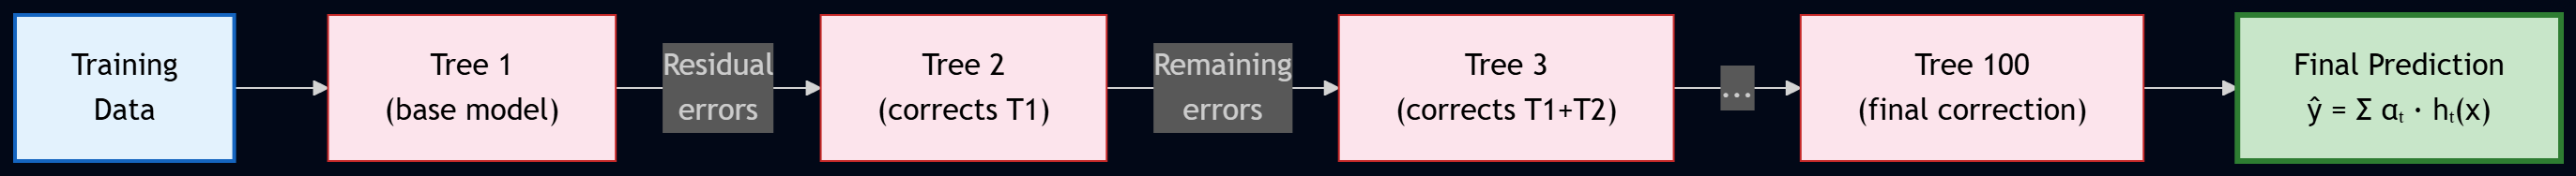
\includegraphics[width=0.95\textwidth]{mermaid_gradient_boosting_concept.png}
    \caption{Conceptual diagram of the Gradient Boosting algorithm. Trees are built sequentially, with each new tree correcting the residual errors of all previous trees. The final prediction is a weighted sum: $\hat{y} = \sum_{t=1}^{T} \alpha_t \cdot h_t(\mathbf{x})$.}
    \label{fig:gb_concept}
\end{figure}

The mathematical formulation for Gradient Boosting is:

\begin{equation}
    \hat{y}(\mathbf{x}) = \sum_{t=1}^{T} \alpha_t \, h_t(\mathbf{x})
    \label{eq:gb}
\end{equation}

\noindent where $\alpha_t$ is the learning rate (shrinkage parameter) and $h_t(\mathbf{x})$ is the $t$-th tree trained on the residuals $r_t = y - \hat{y}_{t-1}(\mathbf{x})$ from the previous ensemble.

Gradient Boosting typically achieves higher accuracy than Random Forest on structured/tabular data, as the sequential error correction mechanism allows it to capture subtle non-linear interactions between features. However, it is more prone to overfitting, particularly on small datasets, and the sequential nature of training means it cannot be parallelised as easily.

In our implementation, we use $T = 100$ trees with a learning rate of $\alpha = 0.1$, maximum tree depth of 3, and \texttt{min\_samples\_leaf=2} to balance model complexity with the small dataset size.

\section{Gaussian Process Regression}
\label{sec:gp}

Gaussian Process (GP) regression is a Bayesian non-parametric approach that models the target function as a realisation of a Gaussian process---a collection of random variables, any finite number of which have a joint Gaussian distribution \citep{rasmussen2006}. Rather than learning fixed model parameters, GP regression maintains a posterior distribution over functions, providing both a mean prediction and an uncertainty estimate for each input.

\begin{figure}[H]
    \centering
    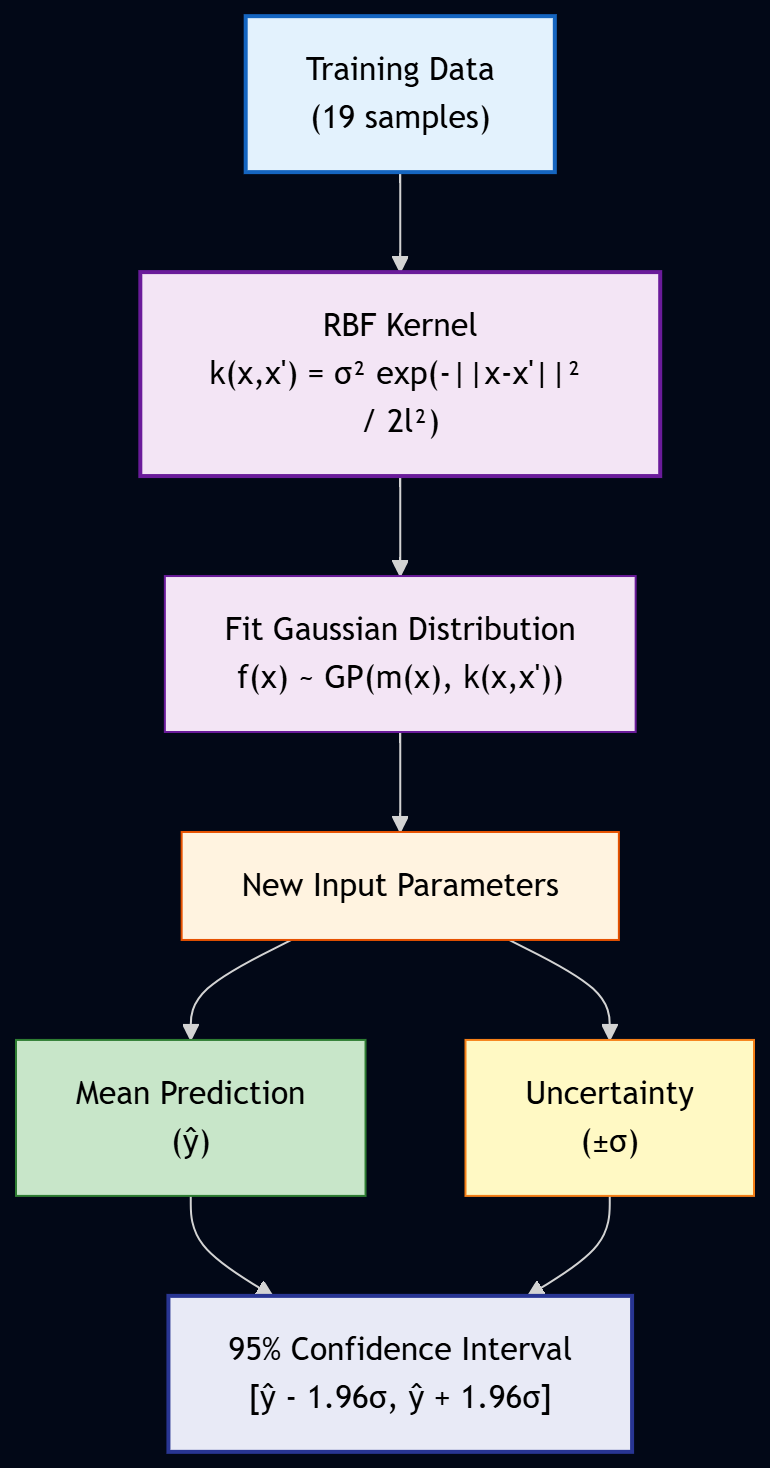
\includegraphics[width=0.55\textwidth]{mermaid_gaussian_process_concept.png}
    \caption{Conceptual diagram of Gaussian Process regression. Training data is used to fit a GP with a composite kernel ($C \cdot \text{RBF} + \text{WhiteKernel}$). For new inputs, the model provides both a mean prediction ($\hat{y}$) and an uncertainty estimate ($\pm\sigma$), yielding a 95\% confidence interval.}
    \label{fig:gp_concept}
\end{figure}

A GP is fully specified by its mean function $m(\mathbf{x})$ and covariance (kernel) function $k(\mathbf{x}, \mathbf{x}')$:

\begin{equation}
    f(\mathbf{x}) \sim \mathcal{GP}\bigl(m(\mathbf{x}),\; k(\mathbf{x}, \mathbf{x}')\bigr)
    \label{eq:gp}
\end{equation}

We employ a composite kernel consisting of a Constant kernel multiplied by an RBF (squared exponential) kernel, plus a White noise kernel:

\begin{equation}
    k(\mathbf{x}, \mathbf{x}') = \sigma_f^2 \exp\!\left(-\frac{\|\mathbf{x} - \mathbf{x}'\|^2}{2\ell^2}\right) + \sigma_n^2 \delta(\mathbf{x}, \mathbf{x}')
    \label{eq:rbf}
\end{equation}

\noindent where $\sigma_f^2$ is the signal variance (ConstantKernel), $\ell$ is the length scale (RBF), and $\sigma_n^2$ is the noise variance (WhiteKernel). All hyperparameters are learned from data by maximising the log marginal likelihood with 10 random restarts (\texttt{n\_restarts\_optimizer=10}). The targets are normalised (\texttt{normalize\_y=True}) to improve numerical stability.

The principal advantage of GP regression for our application is its ability to quantify prediction uncertainty, which is invaluable when the dataset is small ($n = 27$). Points far from the training data receive wide confidence intervals, signalling low confidence and indicating where additional simulations would be most informative. This property is directly exploited in Phase~3, where the GP surrogate drives a Bayesian Optimisation loop using the Expected Improvement acquisition function.

\section{Model Evaluation: Cross-Validation}
\label{sec:cv}

Cross-validation is a resampling technique used to estimate the generalisation performance of a model when an independent test set is not available. For our dataset of $n = 27$ simulations, we employ Leave-One-Out Cross-Validation (LOO~CV), in which each sample is used once as the test set while the remaining $n-1$ samples form the training set. This process is repeated $n$ times, producing one prediction per sample.

\begin{figure}[H]
    \centering
    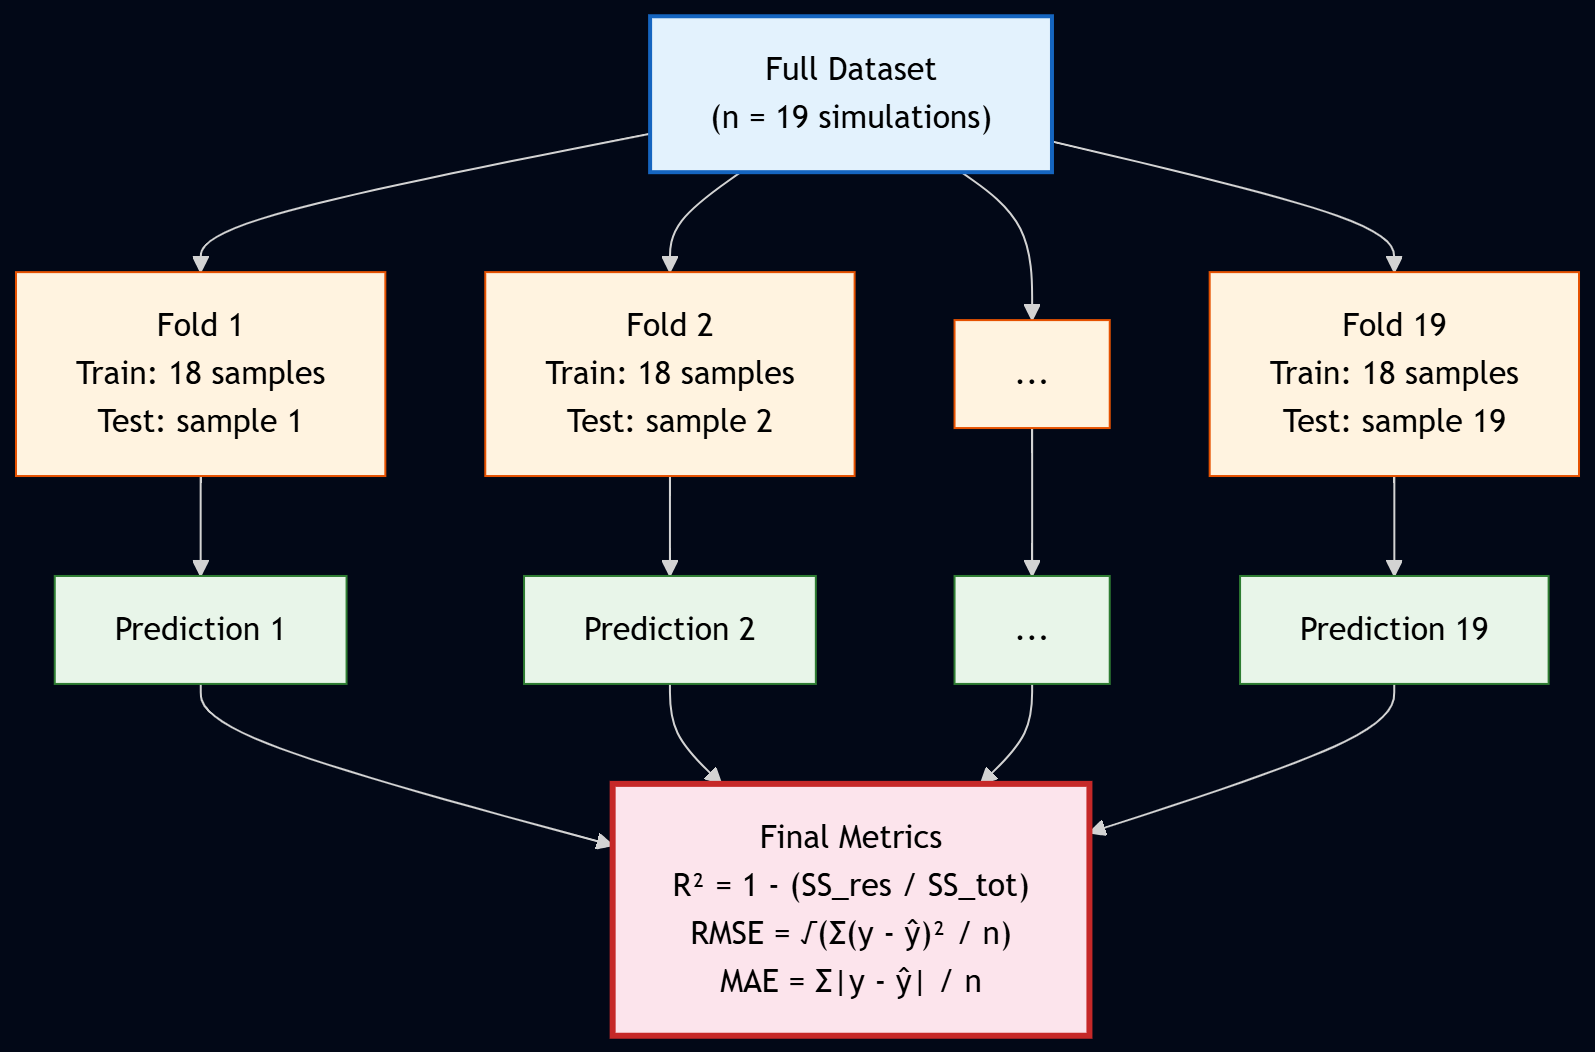
\includegraphics[width=0.7\textwidth]{mermaid_loo_cross_validation.png}
    \caption{Leave-One-Out Cross-Validation (LOO~CV) for $n = 27$ simulations. In each fold, 26 samples are used for training and 1 for testing. The 27 predictions are aggregated to compute the final performance metrics.}
    \label{fig:loo_cv}
\end{figure}

LOO~CV is particularly appropriate for small datasets because it maximises the training set size (using $n-1$ samples), thereby reducing bias in the performance estimate. The three evaluation metrics used are:

\begin{itemize}[leftmargin=2cm]
    \item \textbf{Coefficient of Determination ($R^2$):} Measures the proportion of variance in the target variable explained by the model.
    \begin{equation}
        R^2 = 1 - \frac{\sum_{i=1}^{n}(y_i - \hat{y}_i)^2}{\sum_{i=1}^{n}(y_i - \bar{y})^2}
        \label{eq:r2}
    \end{equation}
    Values range from $-\infty$ to 1, where 1 indicates perfect prediction, 0 indicates performance equal to predicting the mean, and negative values indicate worse-than-mean prediction.

    \item \textbf{Root Mean Squared Error (RMSE):} Measures the average magnitude of prediction errors in the same units as the target.
    \begin{equation}
        \text{RMSE} = \sqrt{\frac{1}{n}\sum_{i=1}^{n}(y_i - \hat{y}_i)^2}
        \label{eq:rmse}
    \end{equation}

    \item \textbf{Mean Absolute Error (MAE):} Measures the average absolute prediction error, less sensitive to outliers than RMSE.
    \begin{equation}
        \text{MAE} = \frac{1}{n}\sum_{i=1}^{n}|y_i - \hat{y}_i|
        \label{eq:mae}
    \end{equation}
\end{itemize}

\section{Summary and Research Gap}
\label{sec:research_gap}

The literature reviewed in this chapter establishes that: (1)~THz metamaterial modulators based on graphene are a promising technology with significant applications; (2)~their design currently relies on time-consuming electromagnetic simulations; and (3)~machine learning surrogates have been successfully applied to accelerate electromagnetic design in related contexts.

However, no existing work has developed an ML surrogate specifically for the graphene metamaterial THz modulator geometry used in this project. Furthermore, existing ML-for-metamaterial studies typically use large datasets ($>$100 simulations), whereas our dataset of 27 simulations presents a unique challenge requiring careful model selection and evaluation.

This project contributes: (a)~an automated data pipeline from COMSOL exports to ML-ready features; (b)~a comparative evaluation of three ML models suited to small datasets; (c)~feature importance analysis linking geometric parameters to physical performance; and (d)~an interactive dashboard for real-time design exploration.


% ============================================================
% CHAPTER 3: SYSTEM DESIGN & IMPLEMENTATION
% ============================================================
\chapter{System Design and Implementation}
\label{ch:design}

In this chapter, I will describe the design and implementation of the system developed for this project. This includes the overall pipeline architecture, the data processing module, the ML training and evaluation framework, and the interactive web dashboard.

\section{System Overview}
\label{sec:system_overview}

The system follows a modular pipeline architecture, as illustrated in Figure~\ref{fig:pipeline}. Raw simulation data from COMSOL Multiphysics is processed through a series of stages, ultimately producing ML predictions and interactive visualisations accessible through a web dashboard.

\begin{figure}[H]
    \centering
    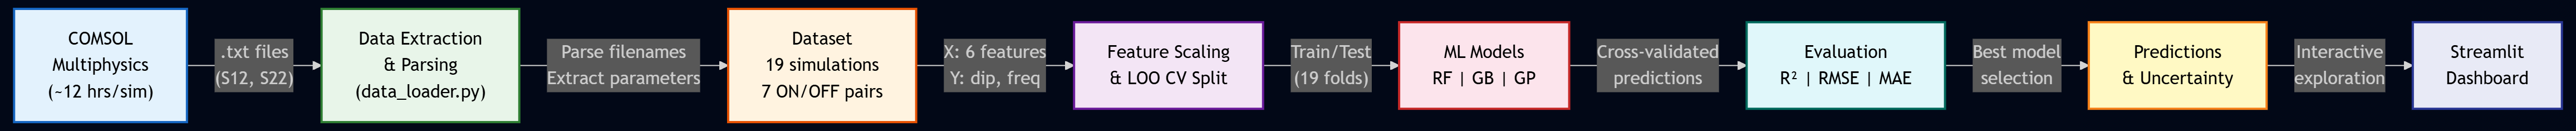
\includegraphics[width=\textwidth]{mermaid_ml_workflow_pipeline.png}
    \caption{End-to-end ML pipeline: COMSOL simulation output files are parsed and processed into a structured dataset, which is split using LOO~CV, used to train three ML models, evaluated on standard metrics, and served through an interactive Streamlit dashboard.}
    \label{fig:pipeline}
\end{figure}

The pipeline consists of six Python modules, all sharing a centralised configuration (\texttt{config.py}) for file paths:

\begin{itemize}[leftmargin=2cm]
    \item \texttt{data\_loader.py} --- Core data pipeline: parsing, parameter extraction, resonance detection, ON/OFF pairing
    \item \texttt{ml\_model.py} --- ML training, LOO~CV evaluation, and prediction
    \item \texttt{streamlit\_app.py} --- Streamlit web dashboard with Plotly interactive charts
    \item \texttt{visualize.py} --- Static matplotlib plot generation
    \item \texttt{analyze.py} --- Sensitivity analysis and text report generation
\end{itemize}

\section{Data Pipeline}
\label{sec:data_pipeline}

The data pipeline, implemented in \texttt{data\_loader.py}, automates the extraction and structuring of simulation data from COMSOL text file exports. This was a critical design decision, as manual data extraction would be error-prone and time-consuming.

\subsection{Filename Parsing}

Simulation parameters are encoded in filenames using a structured naming convention. The general pattern is:

\begin{center}
\texttt{Sdx\{dx\}\_gw\{g\_w\}cw\{c\_w\}wgraph\{w\_graph\}hgraph\{h\_graph\}wau\{w\_au\}\_sigma\{sigma\}.txt}
\end{center}

\noindent For example, \texttt{Sdx35\_gw5cw28wgraph1hgraph2wau4\_sigma0.3.txt} encodes $d_x = 35$, $g_w = 5$, $c_w = 28$, $w_{\text{graph}} = 1$, $h_{\text{graph}} = 2$, $w_{\text{au}} = 4$, and $\sigma = 0.3$~mS.

A regular expression parser handles several edge cases in the naming convention:
\begin{itemize}[leftmargin=2cm]
    \item Files beginning with \texttt{S\_} (no \texttt{dx} prefix) default to $d_x = 35$
    \item Negative parameter values use an \texttt{m} prefix: \texttt{hgraphm6} denotes $h_{\text{graph}} = -6$
    \item Windows download suffixes such as \texttt{(1)}, \texttt{(2)} are automatically stripped
    \item Double underscores (\texttt{\_\_sigma}) are handled gracefully
\end{itemize}

\subsection{S-Parameter Processing}

Each simulation file contains frequency sweep data with columns for frequency (Hz), S12 (dB), and S22 (dB), preceded by \texttt{\%}-prefixed header lines. The parser:
\begin{enumerate}[leftmargin=2cm]
    \item Reads the file, skipping header lines
    \item Extracts frequency and S12 columns
    \item Identifies the resonance dip as the minimum S12 value
    \item Records both the dip depth (dB) and the frequency at which it occurs (GHz)
\end{enumerate}

The filename-based parsing pipeline is designed to be the authoritative source of geometry information, eliminating the risk of transcription errors. Figure~\ref{fig:comsol_params} shows the original COMSOL Parameters pane for one simulation; the values in this pane are what the filename encodes, and the parser reconstructs them exactly.

\begin{figure}[H]
    \centering
    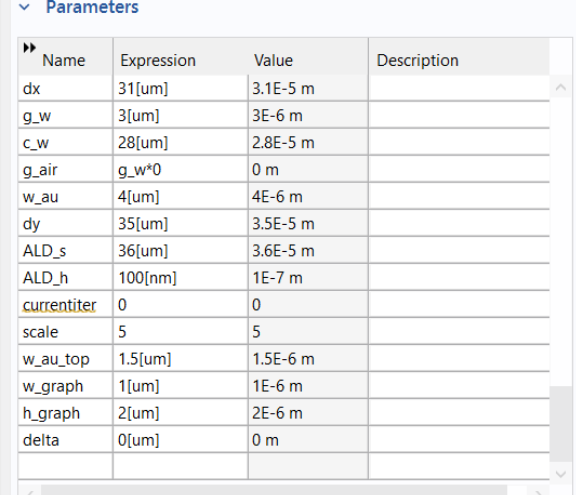
\includegraphics[width=0.6\textwidth]{comsol_parameters_pane.png}
    \caption{COMSOL Parameters pane for a representative simulation (supervisor-provided screenshot, $d_x = 31$~$\mu$m, $g_w = 3$, $c_w = 28$, $h_{\text{graph}} = 2$, $w_{\text{au}} = 4$). The filename parser in \texttt{data\_loader.py} reconstructs every numeric value shown here directly from the exported \texttt{.txt} filename, ensuring the ML training data exactly mirrors what COMSOL computed.}
    \label{fig:comsol_params}
\end{figure}

\subsection{ON/OFF Pairing}

To characterise the modulation performance, ON state ($\sigma = 0.3$~mS) and OFF state ($\sigma = 1.2$~mS) simulations must be paired. The pairing algorithm matches simulations that share identical geometric parameters but differ in conductivity. From the initial 19 simulations, only 7 complete ON/OFF pairs were identified. The Phase~3 data expansion (8 new simulations, including the 5 missing OFF-state counterparts for the $d_x$ sweep) brought the total to 27 simulations and 13 ON/OFF pairs, making modulation-performance ML models substantially more reliable.

\begin{table}[H]
    \centering
    \caption{Example of parsed simulation data showing the mapping from filename parameters to extracted performance metrics.}
    \label{tab:parsed_data}
    \begin{tabular}{cccccc|cc}
        \toprule
        $d_x$ & $g_w$ & $c_w$ & $h_{\text{graph}}$ & $w_{\text{graph}}$ & $w_{\text{au}}$ & S12 Dip (dB) & Dip Freq (GHz) \\
        \midrule
        35 & 3 & 28 & 0 & 1 & 4 & $-14.89$ & 410.0 \\
        35 & 3 & 28 & 6 & 1 & 4 & $-16.64$ & 410.0 \\
        35 & 3 & 28 & $-6$ & 1 & 4 & $-14.95$ & 410.0 \\
        25 & 3 & 28 & 2 & 1 & 4 & $-11.35$ & 500.0 \\
        \bottomrule
    \end{tabular}
\end{table}

\section{ML Training Pipeline}
\label{sec:ml_pipeline}

The ML pipeline, implemented in \texttt{ml\_model.py}, handles feature preparation, model training, cross-validation, and prediction.

\subsection{Feature Engineering}

The feature matrix $\mathbf{X}$ consists of 6 geometric parameters for each simulation, and the target vectors $\mathbf{Y}$ contain the S12 dip depth and resonant frequency:

\begin{equation}
    \mathbf{X} \in \mathbb{R}^{19 \times 6}, \quad \mathbf{Y} \in \mathbb{R}^{19 \times 2}
\end{equation}

All features are standardised using \texttt{StandardScaler} (zero mean, unit variance) before training, which is particularly important for the Gaussian Process model where the RBF kernel is sensitive to feature scales.

\subsection{Model Configuration}

Three models are trained with the following configurations:

\begin{table}[H]
    \centering
    \caption{Hyperparameter configuration for each ML model.}
    \label{tab:hyperparams}
    \begin{tabular}{lll}
        \toprule
        Model & Key Hyperparameters & Library \\
        \midrule
        Random Forest & $T = 100$ trees, \texttt{min\_samples\_leaf=2} & scikit-learn \\
        Gradient Boosting & $T = 100$, $\alpha = 0.1$, \texttt{max\_depth=3} & scikit-learn \\
        Gaussian Process & $C \cdot \text{RBF} + \text{WhiteKernel}$, \texttt{normalize\_y=True} & scikit-learn \\
        \bottomrule
    \end{tabular}
\end{table}

\begin{figure}[H]
    \centering
    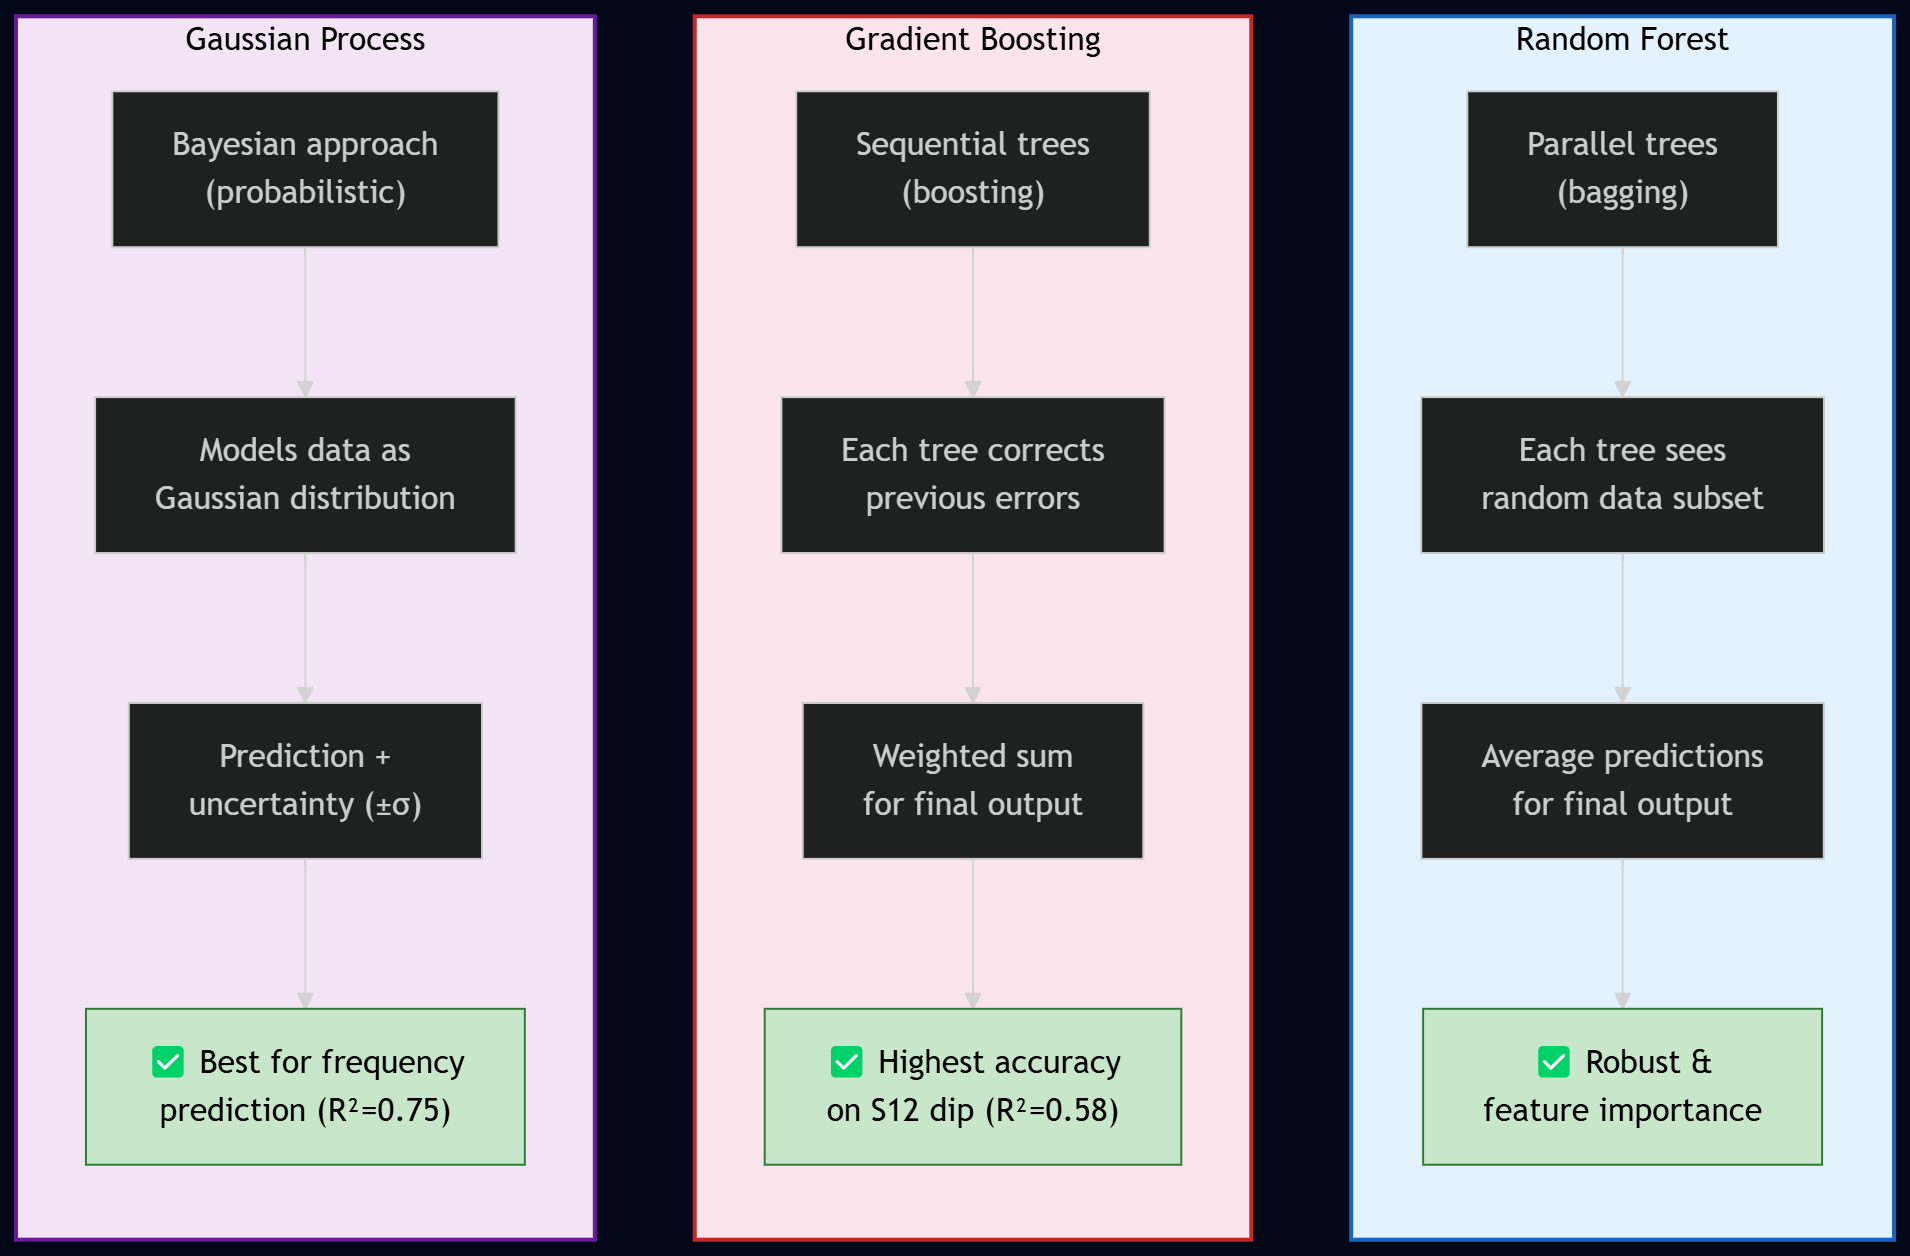
\includegraphics[width=0.9\textwidth]{mermaid_three_models_compared.png}
    \caption{Side-by-side comparison of the three ML models, highlighting their distinct approaches: Random Forest uses parallel bagging, Gradient Boosting uses sequential error correction, and Gaussian Process uses a probabilistic Bayesian framework.}
    \label{fig:three_models}
\end{figure}

\subsection{Leave-One-Out Cross-Validation}

For each of the 19 samples, the model is trained on the remaining 18 and predicts the held-out sample. This yields 19 out-of-sample predictions, from which $R^2$, RMSE, and MAE are computed. This process is repeated independently for each model and each target variable.

\section{Interactive Dashboard}
\label{sec:dashboard}

The interactive dashboard, implemented in \texttt{streamlit\_app.py} using the Streamlit framework with Plotly for interactive charting, provides five pages for data exploration and ML-based prediction.

\subsection{Dashboard Pages}

\begin{enumerate}[leftmargin=2cm]
    \item \textbf{Overview:} Displays key metrics including total simulations, best S12 dip, and best frequency shift, presented as summary cards.
    \item \textbf{Data Explorer:} Interactive table of all 27 simulations with sorting and filtering capabilities.
    \item \textbf{S-Parameter Curves:} Plotly-based interactive plots of S12 transmission curves across all simulations, with hover information showing parameter values.
    \item \textbf{ML Results:} Model performance metrics, actual vs.\ predicted scatter plots, and feature importance bar charts.
    \item \textbf{Predict New Design:} Users input geometric parameters via sliders, and the trained ML models provide instant predictions with a traffic-light confidence indicator (green/amber/red) based on prediction uncertainty.
\end{enumerate}

\begin{figure}[H]
    \centering
    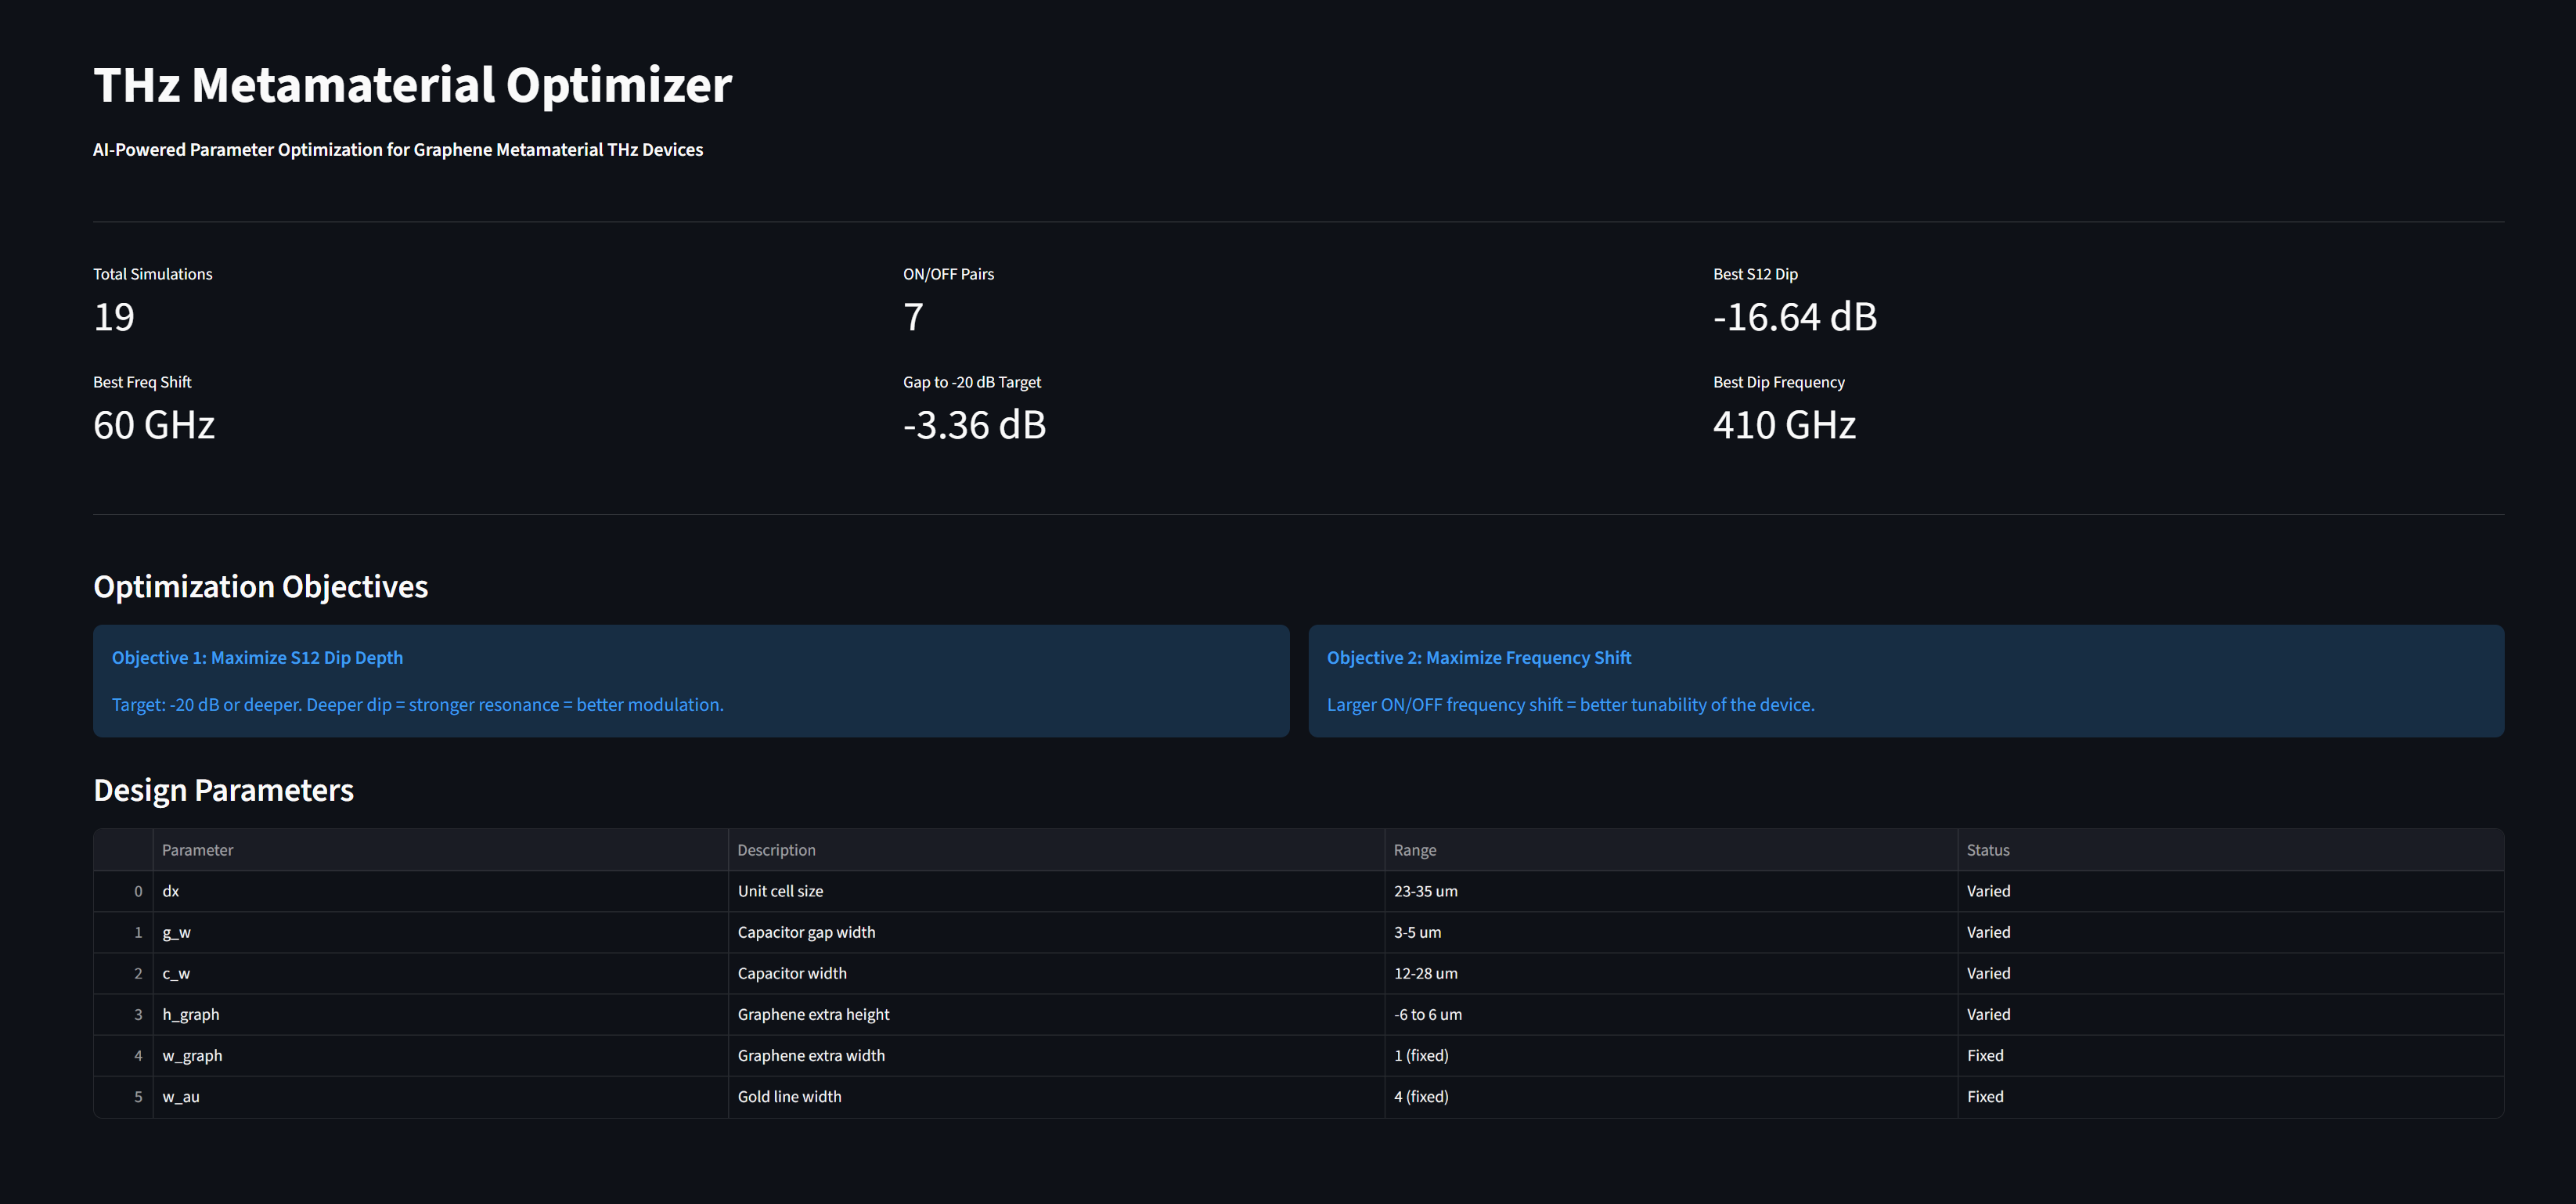
\includegraphics[width=0.9\textwidth]{dashboard_overview.png}
    \caption{Dashboard overview page showing key performance metrics, including total simulations, best S12 dip depth, and summary statistics.}
    \label{fig:dashboard_overview}
\end{figure}

\begin{figure}[H]
    \centering
    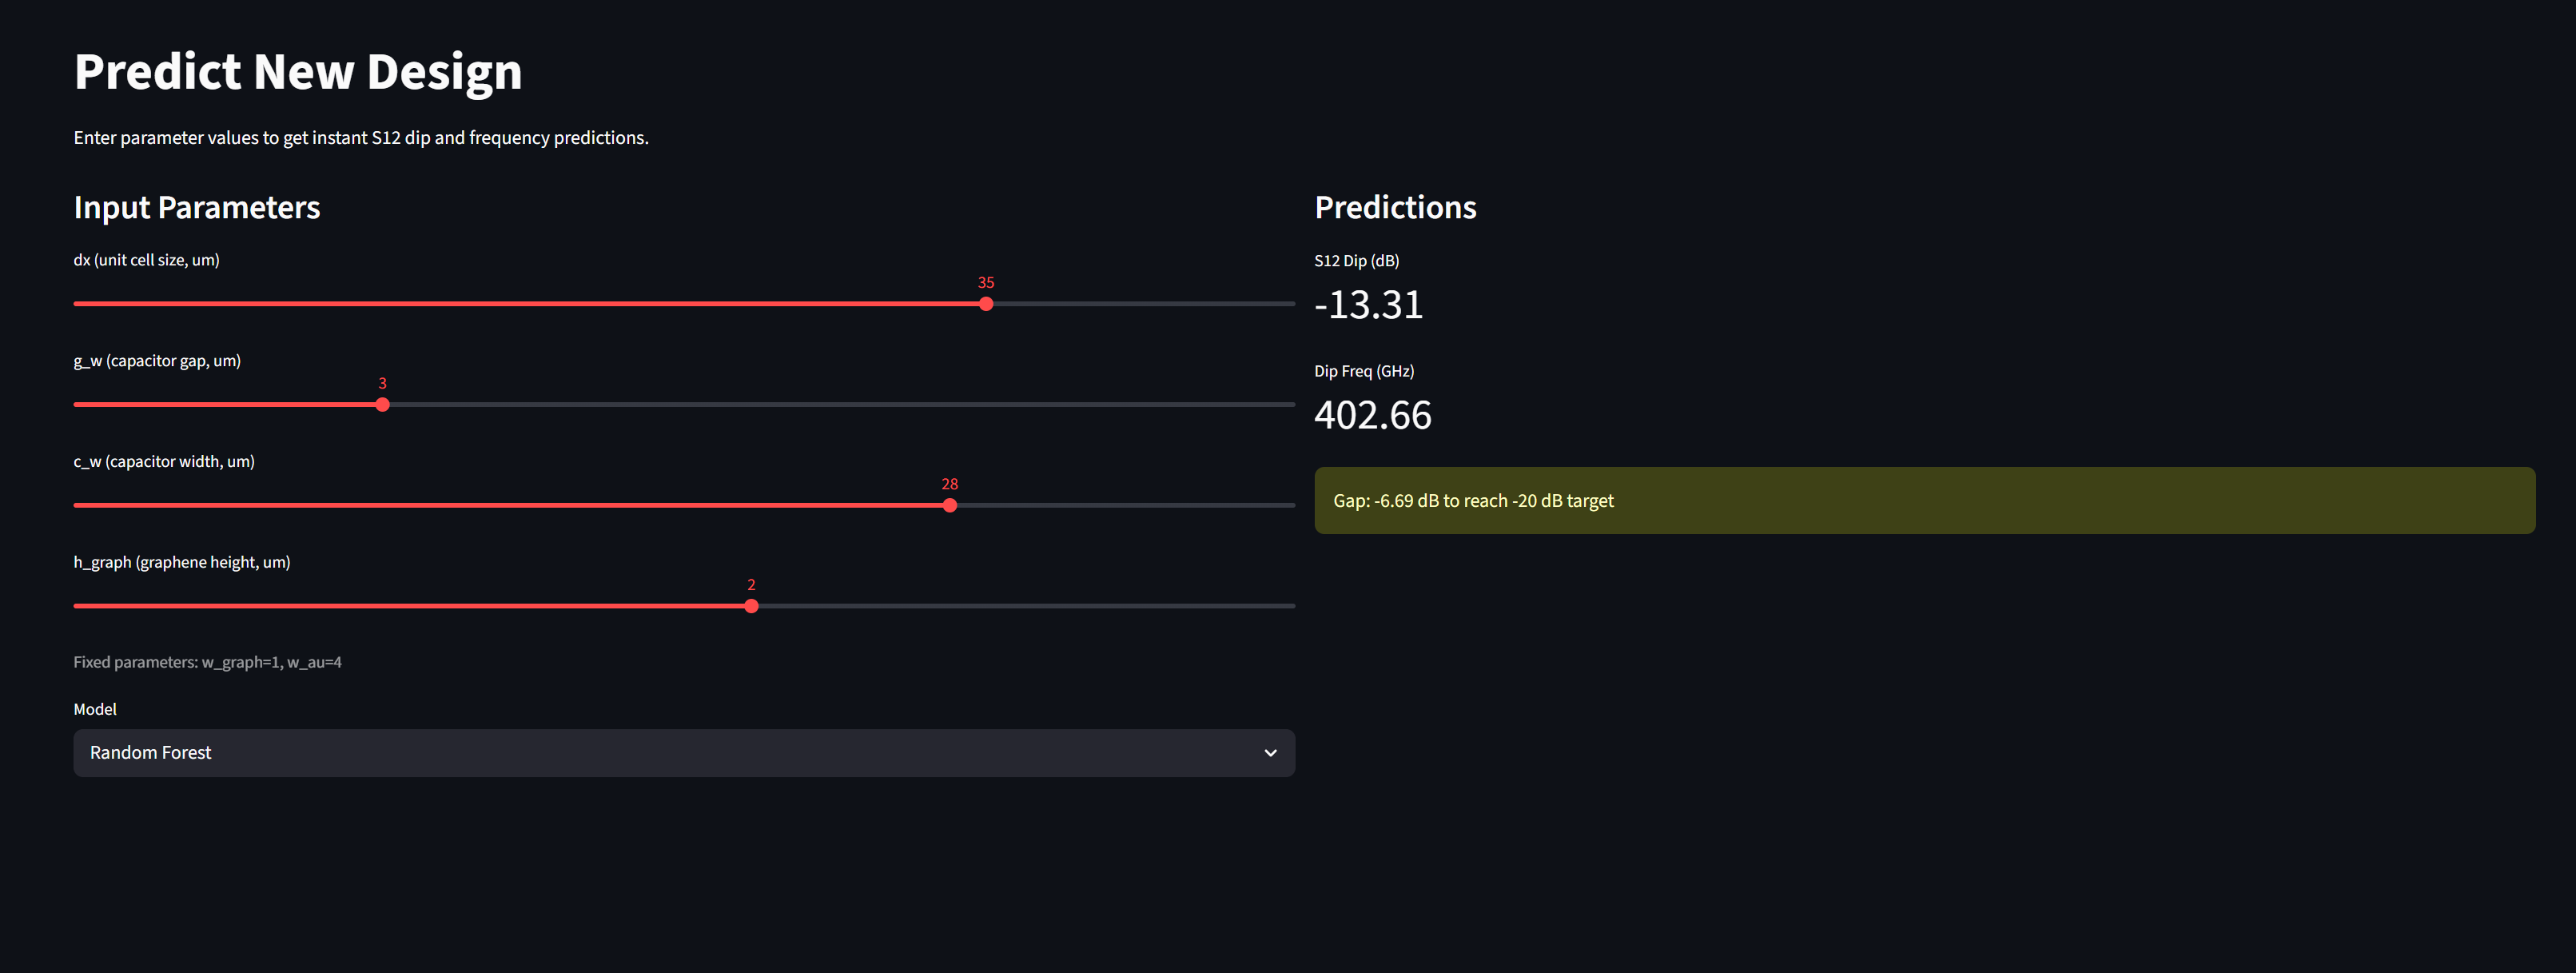
\includegraphics[width=0.9\textwidth]{dashboard_predict_page.png}
    \caption{Prediction page of the dashboard. Users input geometric parameters using sliders, and the ML models provide instant S12 dip and frequency predictions with a traffic-light confidence indicator.}
    \label{fig:dashboard_predict}
\end{figure}

\section{Visualisation and Reporting}
\label{sec:visualisation}

The project employs two complementary visualisation approaches. Static plots are generated using matplotlib with the \texttt{Agg} backend for inclusion in reports, while the dashboard uses Plotly for interactive, browser-based exploration.


% ============================================================
% CHAPTER 4: PHASE 1 — INITIAL DATA COLLECTION
% ============================================================
\chapter{Phase 1: Initial Data Collection and Analysis}
\label{ch:phase1}

In this chapter, I will present the results of Phase~1, which focused on building the initial dataset of 13 COMSOL simulations and performing exploratory data analysis to understand the parameter space.

\section{Simulation Parameters}
\label{sec:phase1_params}

Phase~1 consisted of 13 simulations exploring three geometric parameters while keeping the others fixed:

\begin{itemize}[leftmargin=2cm]
    \item \textbf{$d_x$ (unit cell size):} Varied across 23, 25, 27, 31, 33, and 35~$\mu$m
    \item \textbf{$g_w$ (gap width):} Varied across 3 and 5~$\mu$m
    \item \textbf{$c_w$ (capacitor width):} Varied across 12, 20, and 28~$\mu$m
    \item \textbf{Fixed parameters:} $h_{\text{graph}} = 2$, $w_{\text{graph}} = 1$, $w_{\text{au}} = 4$~$\mu$m
\end{itemize}

All simulations were performed in COMSOL Multiphysics, each requiring approximately 12 hours of computation time on a standard workstation. Both ON ($\sigma = 0.3$~mS) and OFF ($\sigma = 1.2$~mS) states were simulated where possible, though 5 simulations in the $d_x$ sweep were only performed in the ON state.

\section{Phase 1 Results}
\label{sec:phase1_results}

The key findings from Phase~1 are summarised below:

\begin{itemize}[leftmargin=2cm]
    \item \textbf{Best S12 dip:} $-13.41$~dB, achieved with $d_x = 35$, $g_w = 3$, $c_w = 28$---still significantly short of the $-20$~dB target.
    \item \textbf{Parameter sensitivity:} $c_w$ (capacitor width) showed the strongest influence on resonant frequency, while $d_x$ (unit cell size) primarily affected the dip depth.
    \item \textbf{ON/OFF pairing:} 7 complete pairs were identified from the 13 simulations, enabling preliminary analysis of modulation performance.
\end{itemize}

\begin{figure}[H]
    \centering
    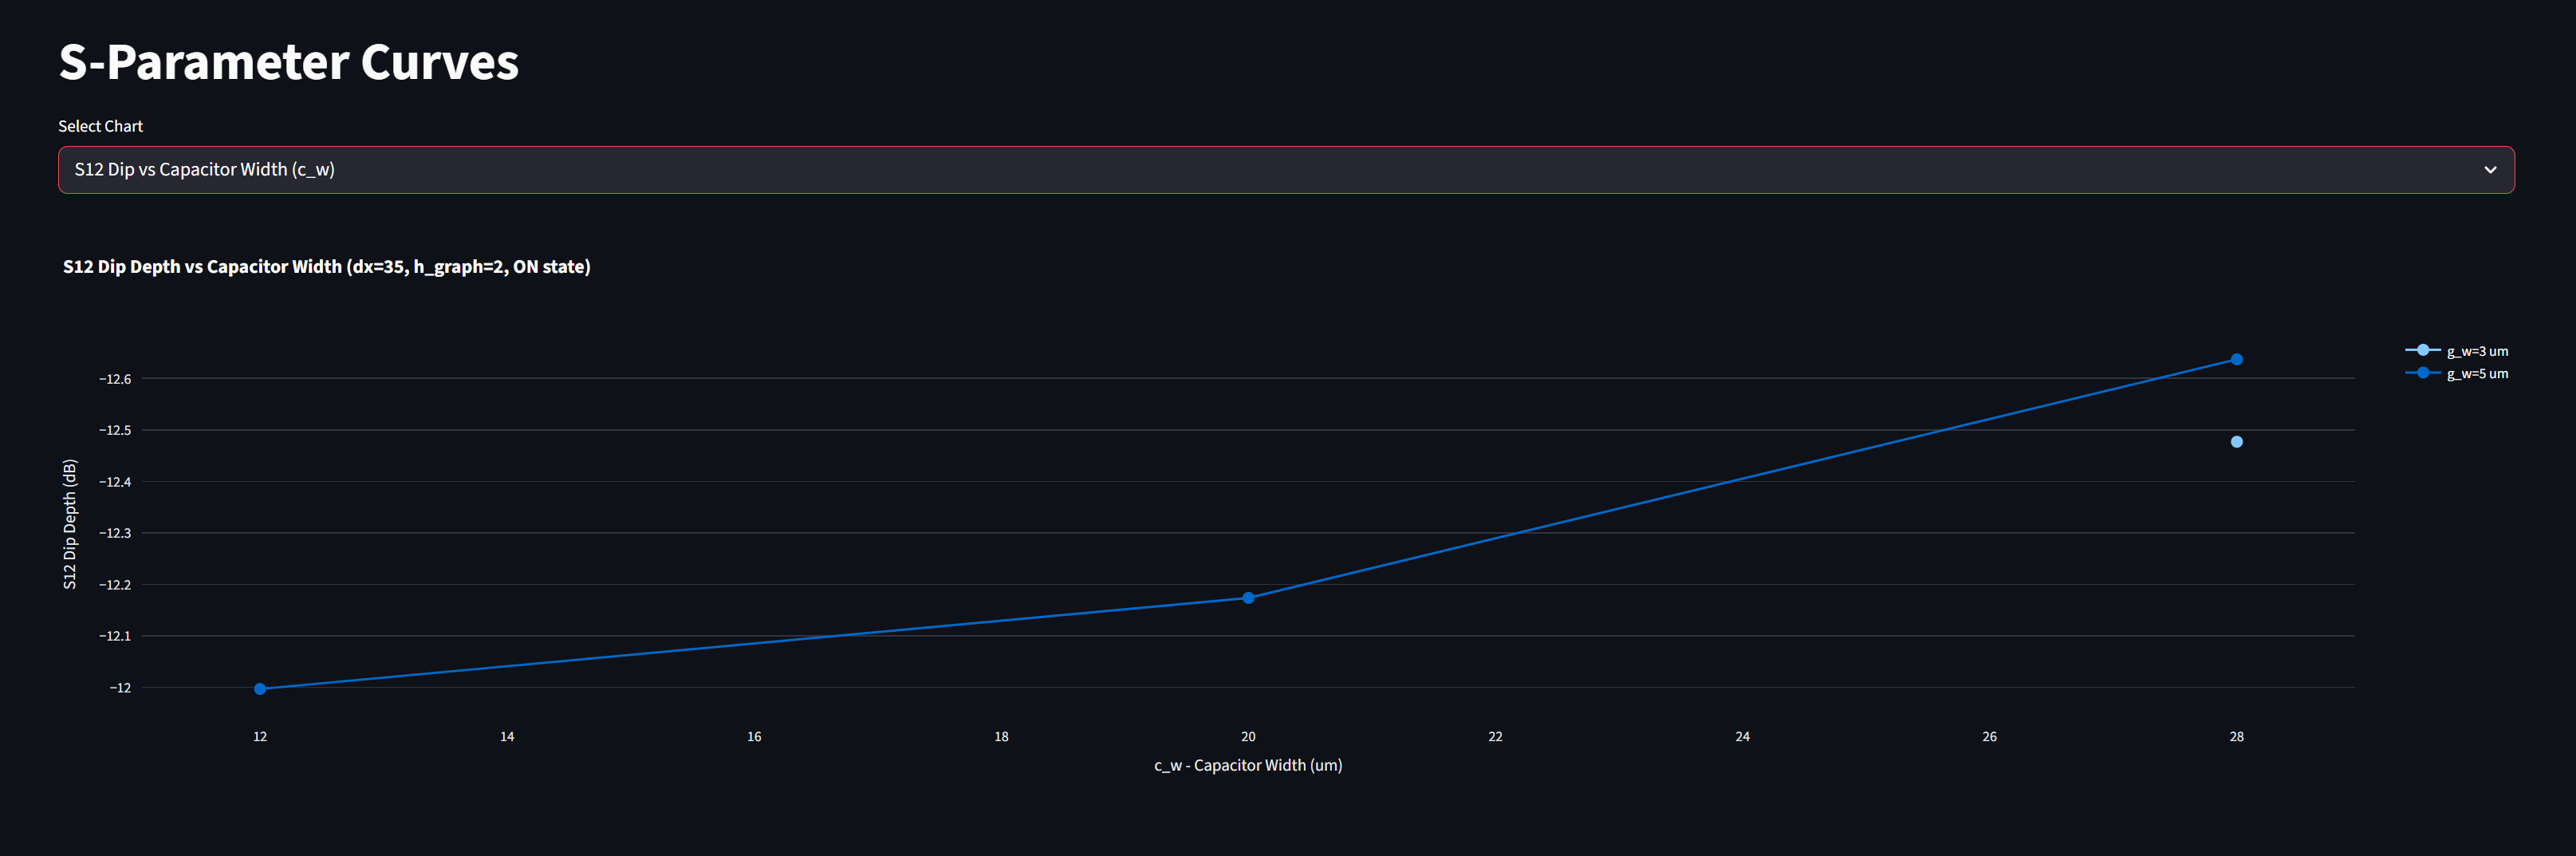
\includegraphics[width=0.85\textwidth]{dashboard_dip_vs_cw.png}
    \caption{Relationship between capacitor width ($c_w$) and S12 dip depth, showing that $c_w$ primarily influences the resonant frequency rather than the dip depth. Data from the interactive dashboard.}
    \label{fig:dip_vs_cw}
\end{figure}

The supervisor independently produced the overlay plot in Figure~\ref{fig:supervisor_gw5} directly from COMSOL, showing three $c_w$ values (12, 20, 28~$\mu$m) at $d_x = 35$, $g_w = 5$. The S12 resonance shifts monotonically from $\sim$600~GHz at $c_w = 12$ down to $\sim$450~GHz at $c_w = 28$, exactly the inverse-square-root behaviour predicted by the equivalent LC circuit model ($f \propto 1/\sqrt{LC}$, $C \propto c_w$). This visual confirmation of the dashboard trend (Figure~\ref{fig:dip_vs_cw}) validates the parsing pipeline end-to-end: the dashboard plot is generated from parsed \texttt{.txt} files, and it reproduces the same trend the supervisor saw directly in COMSOL.

\begin{figure}[H]
    \centering
    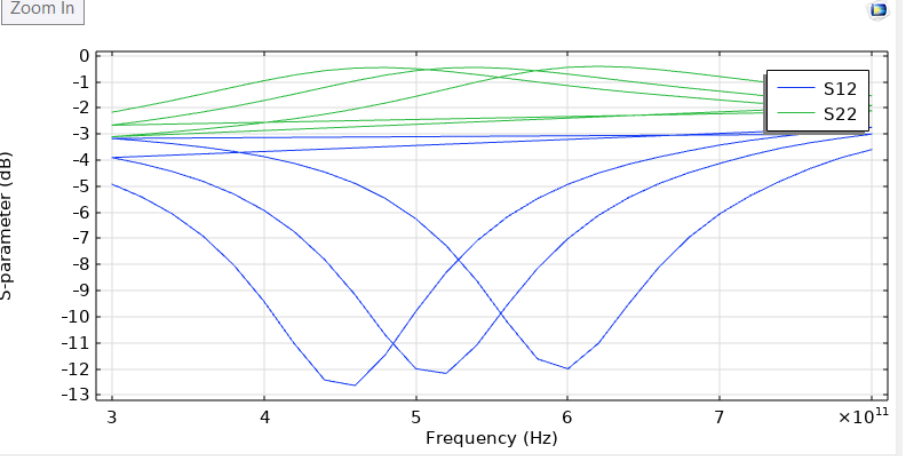
\includegraphics[width=0.85\textwidth]{supervisor_gw5_cw_sweep.png}
    \caption{Supervisor-provided COMSOL overlay of three Phase~1 simulations at $d_x = 35$, $g_w = 5$, with $c_w \in \{12, 20, 28\}$~$\mu$m (all at $\sigma = 0.3$~mS). The three S12 dips shift monotonically with $c_w$, confirming the $f \propto 1/\sqrt{c_w}$ scaling captured in the ML model's feature-importance analysis (Section~\ref{sec:feature_importance}).}
    \label{fig:supervisor_gw5}
\end{figure}

\begin{figure}[H]
    \centering
    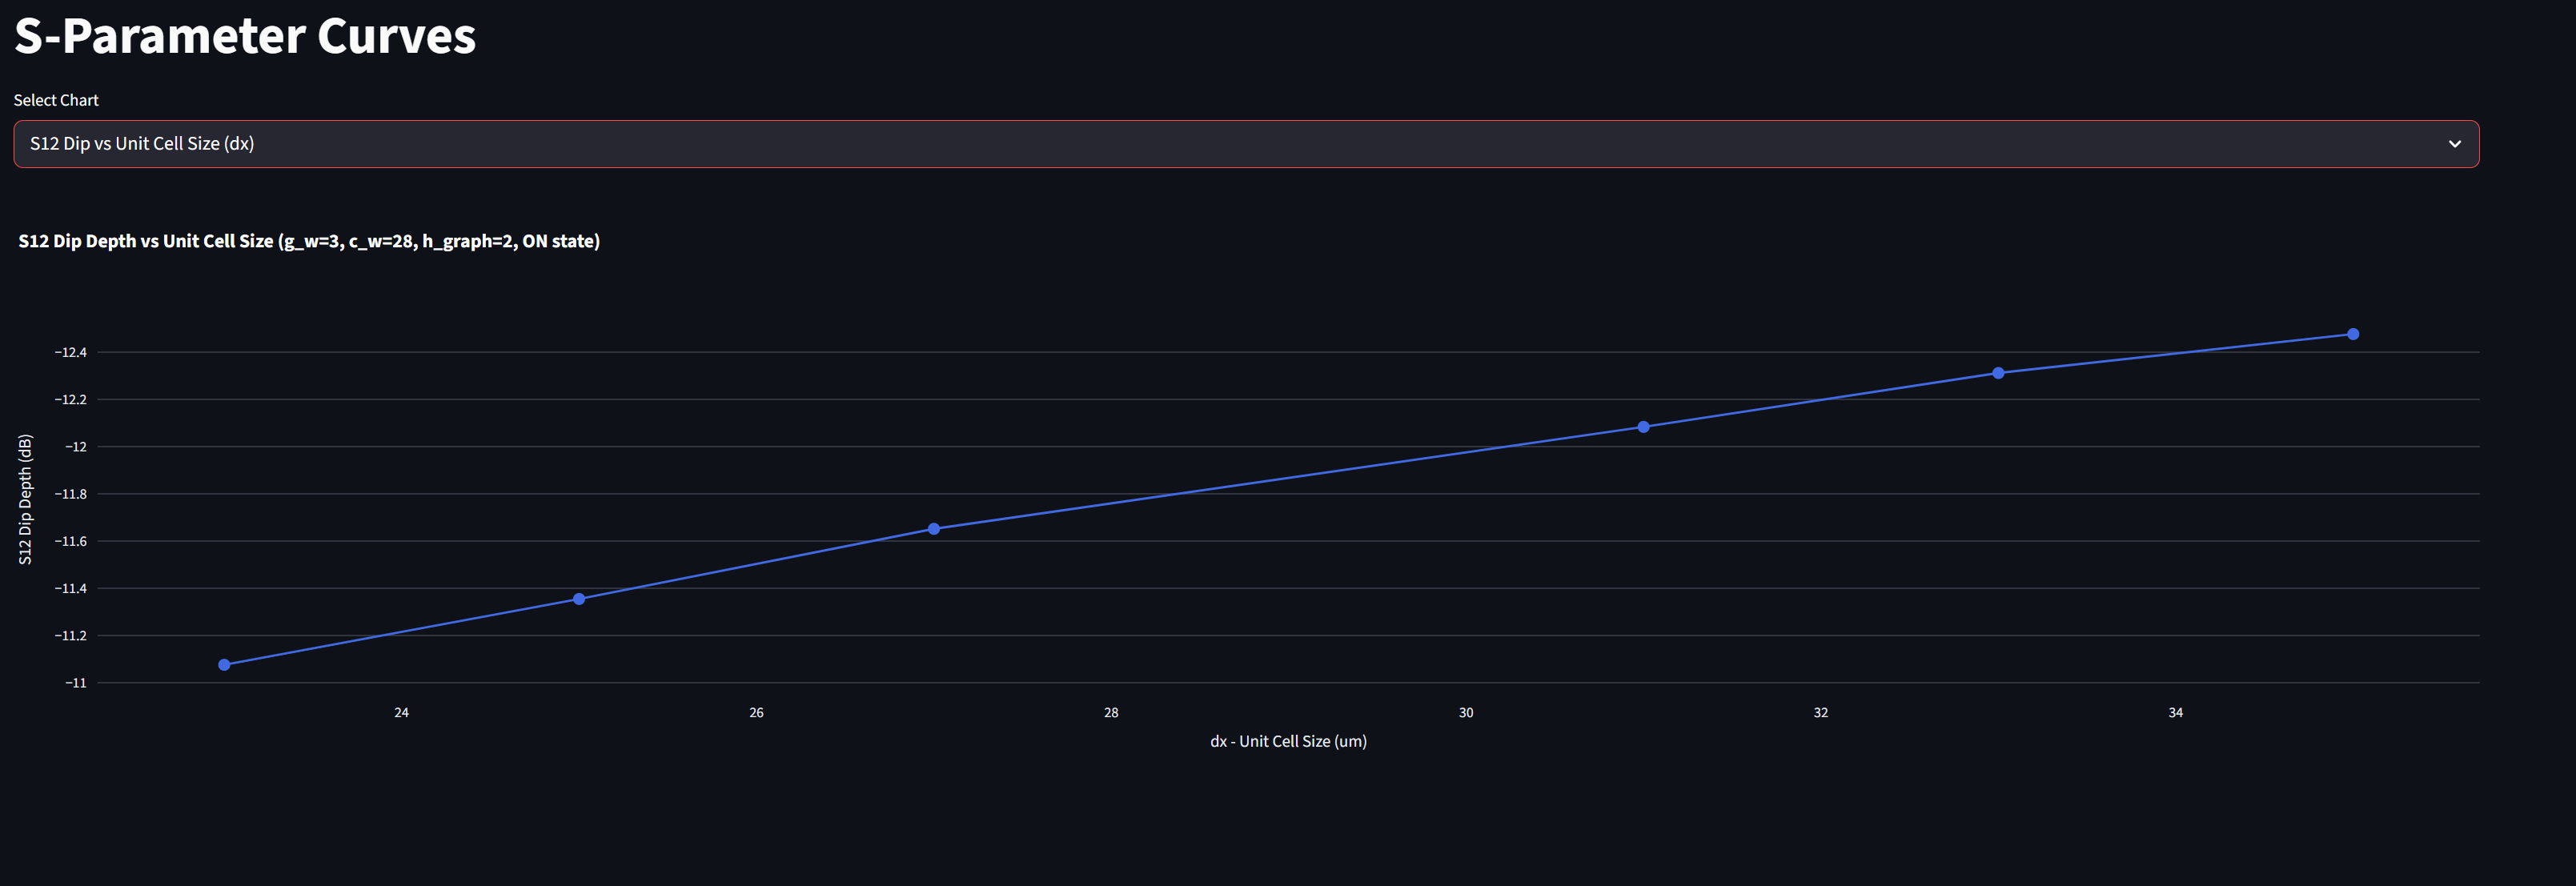
\includegraphics[width=0.85\textwidth]{dashboard_dip_vs_dx.png}
    \caption{Relationship between unit cell size ($d_x$) and S12 dip depth, showing a general trend of deeper dips with larger unit cells. Data from the interactive dashboard.}
    \label{fig:dip_vs_dx}
\end{figure}

\section{Observations and Limitations}
\label{sec:phase1_limitations}

Phase~1 established the data pipeline and provided initial insights into parameter sensitivity, but several limitations were identified:

\begin{enumerate}[leftmargin=2cm]
    \item \textbf{Limited parameter exploration:} Only three of seven parameters were varied, leaving the influence of $h_{\text{graph}}$, $w_{\text{graph}}$, $w_{\text{au}}$, and $w_{\text{au,top}}$ unexplored.
    \item \textbf{No ML models:} Analysis was limited to manual inspection and basic visualisation.
    \item \textbf{Missing OFF-state data:} Five simulations lacked OFF-state counterparts, limiting the modulation analysis.
    \item \textbf{Insufficient dip depth:} The best achieved dip of $-13.41$~dB remained 6.59~dB short of the $-20$~dB target, indicating that the explored region of parameter space had not yet reached optimal performance.
\end{enumerate}

These observations motivated the Phase~2 work: expanding the dataset to include $h_{\text{graph}}$ variation and implementing ML models for systematic analysis and prediction.


% ============================================================
% CHAPTER 5: PHASE 2 — EXPANDED DATASET & ML RESULTS
% ============================================================
\chapter{Phase 2: Expanded Dataset and ML Results}
\label{ch:phase2}

In this chapter, I will present the Phase~2 and Phase~3 results, including the expanded simulation dataset, ML model evaluation across all 27 simulations and the 13 ON/OFF pairs, feature importance analysis, and a demonstration of the interactive dashboard.

\section{New Simulations}
\label{sec:new_sims}

Phase~2 added 6 new COMSOL simulations to the dataset, specifically targeting unexplored values of the $h_{\text{graph}}$ parameter. While Phase~1 used $h_{\text{graph}} = 2$ throughout, Phase~2 introduced $h_{\text{graph}} \in \{-6, 0, 6\}$ while keeping other parameters at their baseline values ($d_x = 35$, $g_w = 3$, $c_w = 28$). Both ON ($\sigma = 0.3$~mS) and OFF ($\sigma = 1.2$~mS) states were simulated, bringing the dataset to 19 simulations.

Phase~3 further expanded the dataset with 8 additional simulations provided by the supervisor: 5 missing OFF-state counterparts for the $d_x$ sweep (at $d_x \in \{23, 25, 27, 31, 33\}$), plus 3 simulations introducing variance in the previously-fixed gold width parameter, $w_{\text{au}} \in \{3, 5\}$, alongside a new $h_{\text{graph}} = -2$ configuration. This brought the total to 27 simulations and 13 ON/OFF pairs, and critically resolved the zero-variance artefact that had made Phase~2's feature importance analysis for $w_{\text{au}}$ uninformative.

The most significant discovery of Phase~2 was that $h_{\text{graph}} = 6$ produced an S12 dip of $-16.64$~dB---a substantial improvement of 3.23~dB over the Phase~1 best of $-13.41$~dB. This brought the design to within 3.36~dB of the $-20$~dB target, demonstrating that graphene thickness offset is a critical parameter for optimising dip depth.

\begin{figure}[H]
    \centering
    \begin{subfigure}[b]{0.48\textwidth}
        \centering
        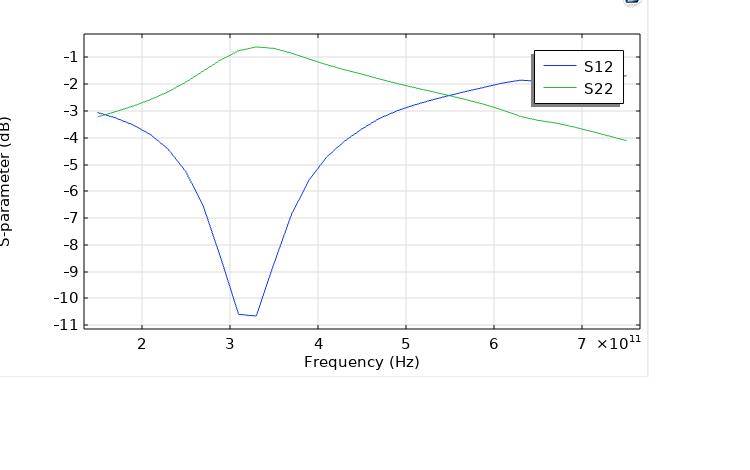
\includegraphics[width=\textwidth]{comsol_sparam_on_state.jpeg}
        \caption{ON state ($\sigma = 0.3$~mS)}
        \label{fig:sparam_on}
    \end{subfigure}
    \hfill
    \begin{subfigure}[b]{0.48\textwidth}
        \centering
        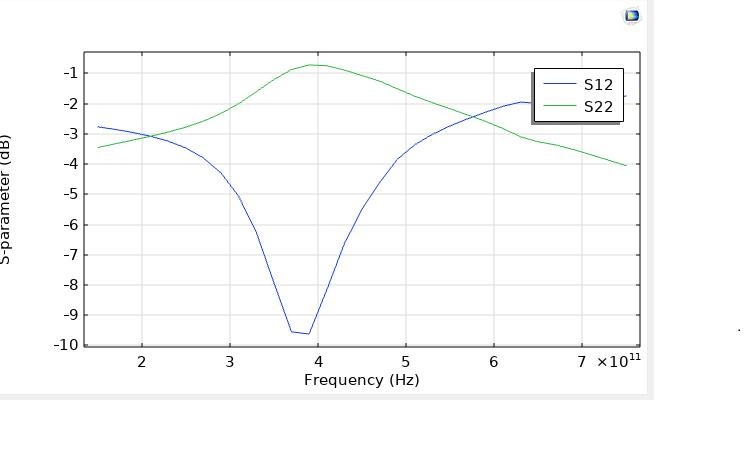
\includegraphics[width=\textwidth]{comsol_sparam_off_state.jpeg}
        \caption{OFF state ($\sigma = 1.2$~mS)}
        \label{fig:sparam_off}
    \end{subfigure}
    \caption{Typical COMSOL S-parameter response showing S12 (transmission) and S22 (reflection) curves. The ON state (a) shows the characteristic transmission dip, while the OFF state (b) shows the shifted response due to increased graphene conductivity.}
    \label{fig:sparam_comparison}
\end{figure}

Figure~\ref{fig:supervisor_hgraph} shows the supervisor's direct overlay of the Phase~2 $h_{\text{graph}}$ sweep: all simulations share $d_x = 35$, $g_w = 3$, $c_w = 28$, $w_{\text{au}} = 4$, $\sigma = 0.3$~mS, varying only $h_{\text{graph}}$. The two overlaid S12 curves show that even small changes in graphene thickness offset shift the resonance by $\sim$20~GHz and change the dip depth by more than 1~dB. This is the direct COMSOL evidence behind the $h_{\text{graph}} = 6$ discovery that drives the $-16.64$~dB record dip, and it also justifies retaining $h_{\text{graph}}$ as a key feature in the ML model despite its reduced dominance (importance $\sim$0.25) after the Phase~3 expansion.

\begin{figure}[H]
    \centering
    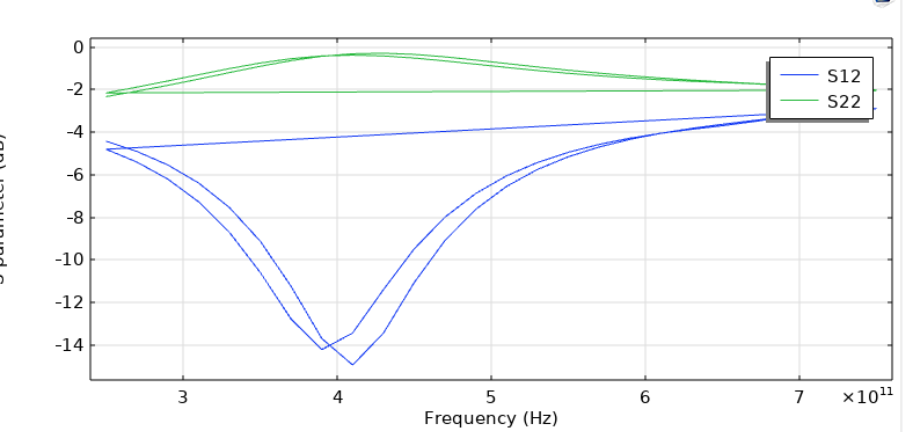
\includegraphics[width=0.8\textwidth]{supervisor_hgraph_sweep.png}
    \caption{Supervisor-provided COMSOL overlay of the $h_{\text{graph}}$ sweep at baseline geometry ($d_x = 35$, $g_w = 3$, $c_w = 28$, $w_{\text{au}} = 4$). Different values of $h_{\text{graph}}$ produce visibly different dip depths and resonance positions, demonstrating that graphene thickness offset materially affects the device response even within the narrow range explored here.}
    \label{fig:supervisor_hgraph}
\end{figure}

The Phase~3 data expansion introduced variance in $w_{\text{au}}$ for the first time. Figure~\ref{fig:supervisor_wau} shows the supervisor's overlay of $w_{\text{au}}$ variations at fixed geometry ($d_x = 35$, $g_w = 3$, $c_w = 28$, $h_{\text{graph}} = -2$), confirming that the gold width produces a measurable but comparatively modest change in the S-parameter response --- consistent with the ML feature importance of 0.049 that emerged only after these simulations were added to the training set (Section~\ref{sec:feature_importance}).

\begin{figure}[H]
    \centering
    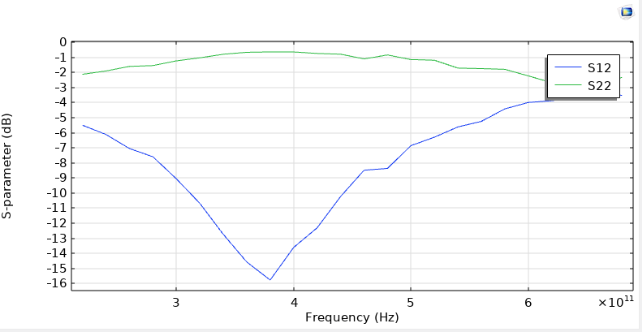
\includegraphics[width=0.8\textwidth]{supervisor_wau_sweep.png}
    \caption{Supervisor-provided COMSOL overlay for the Phase~3 $w_{\text{au}}$ sweep at $d_x = 35$, $g_w = 3$, $c_w = 28$, $h_{\text{graph}} = -2$. The curves differ only slightly with $w_{\text{au}}$, consistent with the small-but-non-zero feature importance (0.049) that the ML model assigns to this parameter.}
    \label{fig:supervisor_wau}
\end{figure}

A final set of Phase~3 simulations completed the 5 missing OFF-state counterparts for the original $d_x$ sweep ($d_x \in \{23, 25, 27, 31, 33\}$ at $\sigma = 1.2$~mS). Figure~\ref{fig:supervisor_dx_off} shows the supervisor's overlay of these newly-added simulations. This single supervisor-provided batch is directly responsible for increasing the ON/OFF pair count from 7 to 13, transforming the pair-based ML models from ``failing'' ($R^2 < 0$ for GP) to ``viable'' ($R^2 = 0.47$ for RF on frequency shift).

\begin{figure}[H]
    \centering
    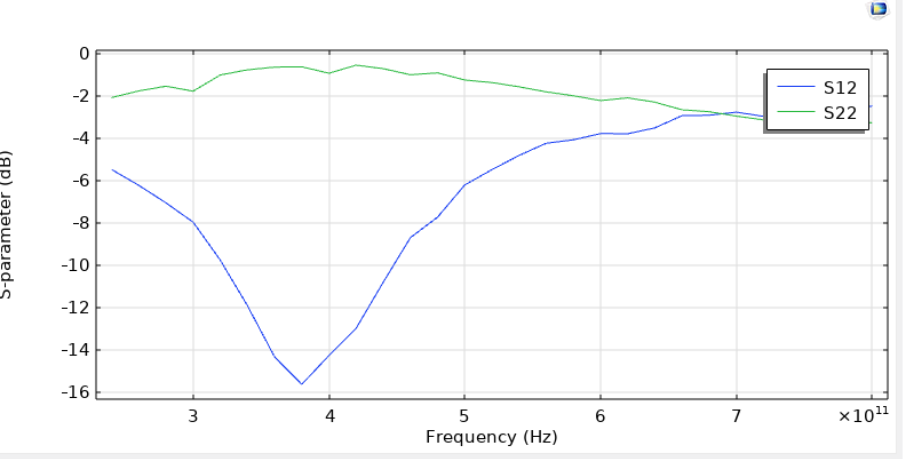
\includegraphics[width=0.8\textwidth]{supervisor_dx_sweep_off.png}
    \caption{Supervisor-provided COMSOL overlay of the 5 newly-added OFF-state simulations ($d_x \in \{23, 25, 27, 31, 33\}$, $\sigma = 1.2$~mS). These simulations completed the ON/OFF pairing for the full $d_x$ sweep and were critical in bringing the pair-based ML models into a usable regime.}
    \label{fig:supervisor_dx_off}
\end{figure}

\section{ML Model Evaluation: All 19 Simulations}
\label{sec:ml_all}

Three ML models were trained and evaluated using LOO~CV on the complete dataset of 27 simulations. Table~\ref{tab:ml_all} presents the full evaluation metrics for both target variables.

\begin{table}[H]
    \centering
    \caption{ML model performance on all 27 simulations using LOO cross-validation. Bold values indicate the best performance for each metric. Relative to the Phase~2 snapshot ($n=19$), primary-target $R^2$ values dropped as the expanded parameter space (introducing $w_{\text{au}}$ and $h_{\text{graph}}=-2$ variance) revealed the Phase~2 models had been operating in a narrower, easier regime.}
    \label{tab:ml_all}
    \begin{tabular}{ll|ccc}
        \toprule
        Target & Model & $R^2$ & RMSE & MAE \\
        \midrule
        \multirow{3}{*}{S12 Dip (dB)}
        & Random Forest     & $-0.020$ & 1.700 & 1.409 \\
        & Gradient Boosting & $-0.328$ & 1.940 & 1.620 \\
        & Gaussian Process  & \textbf{0.078} & \textbf{1.617} & \textbf{1.341} \\
        \midrule
        \multirow{3}{*}{Dip Freq (GHz)}
        & Random Forest     & 0.536 & 41.55 & 33.54 \\
        & Gradient Boosting & 0.495 & 43.34 & 38.07 \\
        & Gaussian Process  & \textbf{0.681} & \textbf{34.42} & \textbf{29.53} \\
        \bottomrule
    \end{tabular}
\end{table}

Key observations from Table~\ref{tab:ml_all}:
\begin{itemize}[leftmargin=2cm]
    \item \textbf{Gaussian Process} achieves the best performance on both targets ($R^2 = 0.078$ for S12 dip, $R^2 = 0.681$ for frequency), consistent with its theoretical strength on smooth, low-sample-count regression problems.
    \item \textbf{S12 dip prediction is now substantially harder than Phase~2 suggested.} All three models struggle ($R^2 \leq 0.08$), with Gradient Boosting actually producing negative $R^2$ on this target. This is a direct consequence of introducing real variance in $w_{\text{au}}$ and adding the $h_{\text{graph}} = -2$ configuration: the model must now learn across a wider, less homogeneous parameter space. The Phase~2 $R^2$ of 0.58 was artificially high because the training data occupied a narrower slice.
    \item \textbf{Dip frequency prediction remains strong.} Gaussian Process maintains $R^2 = 0.68$, only marginally below the Phase~2 value of 0.75, indicating that the resonant frequency depends smoothly on geometry in a way that generalises well across the expanded dataset.
    \item \textbf{Random Forest} serves as a robust baseline and provides the most trustworthy feature importance rankings in Section~\ref{sec:feature_importance}.
\end{itemize}

\begin{figure}[H]
    \centering
    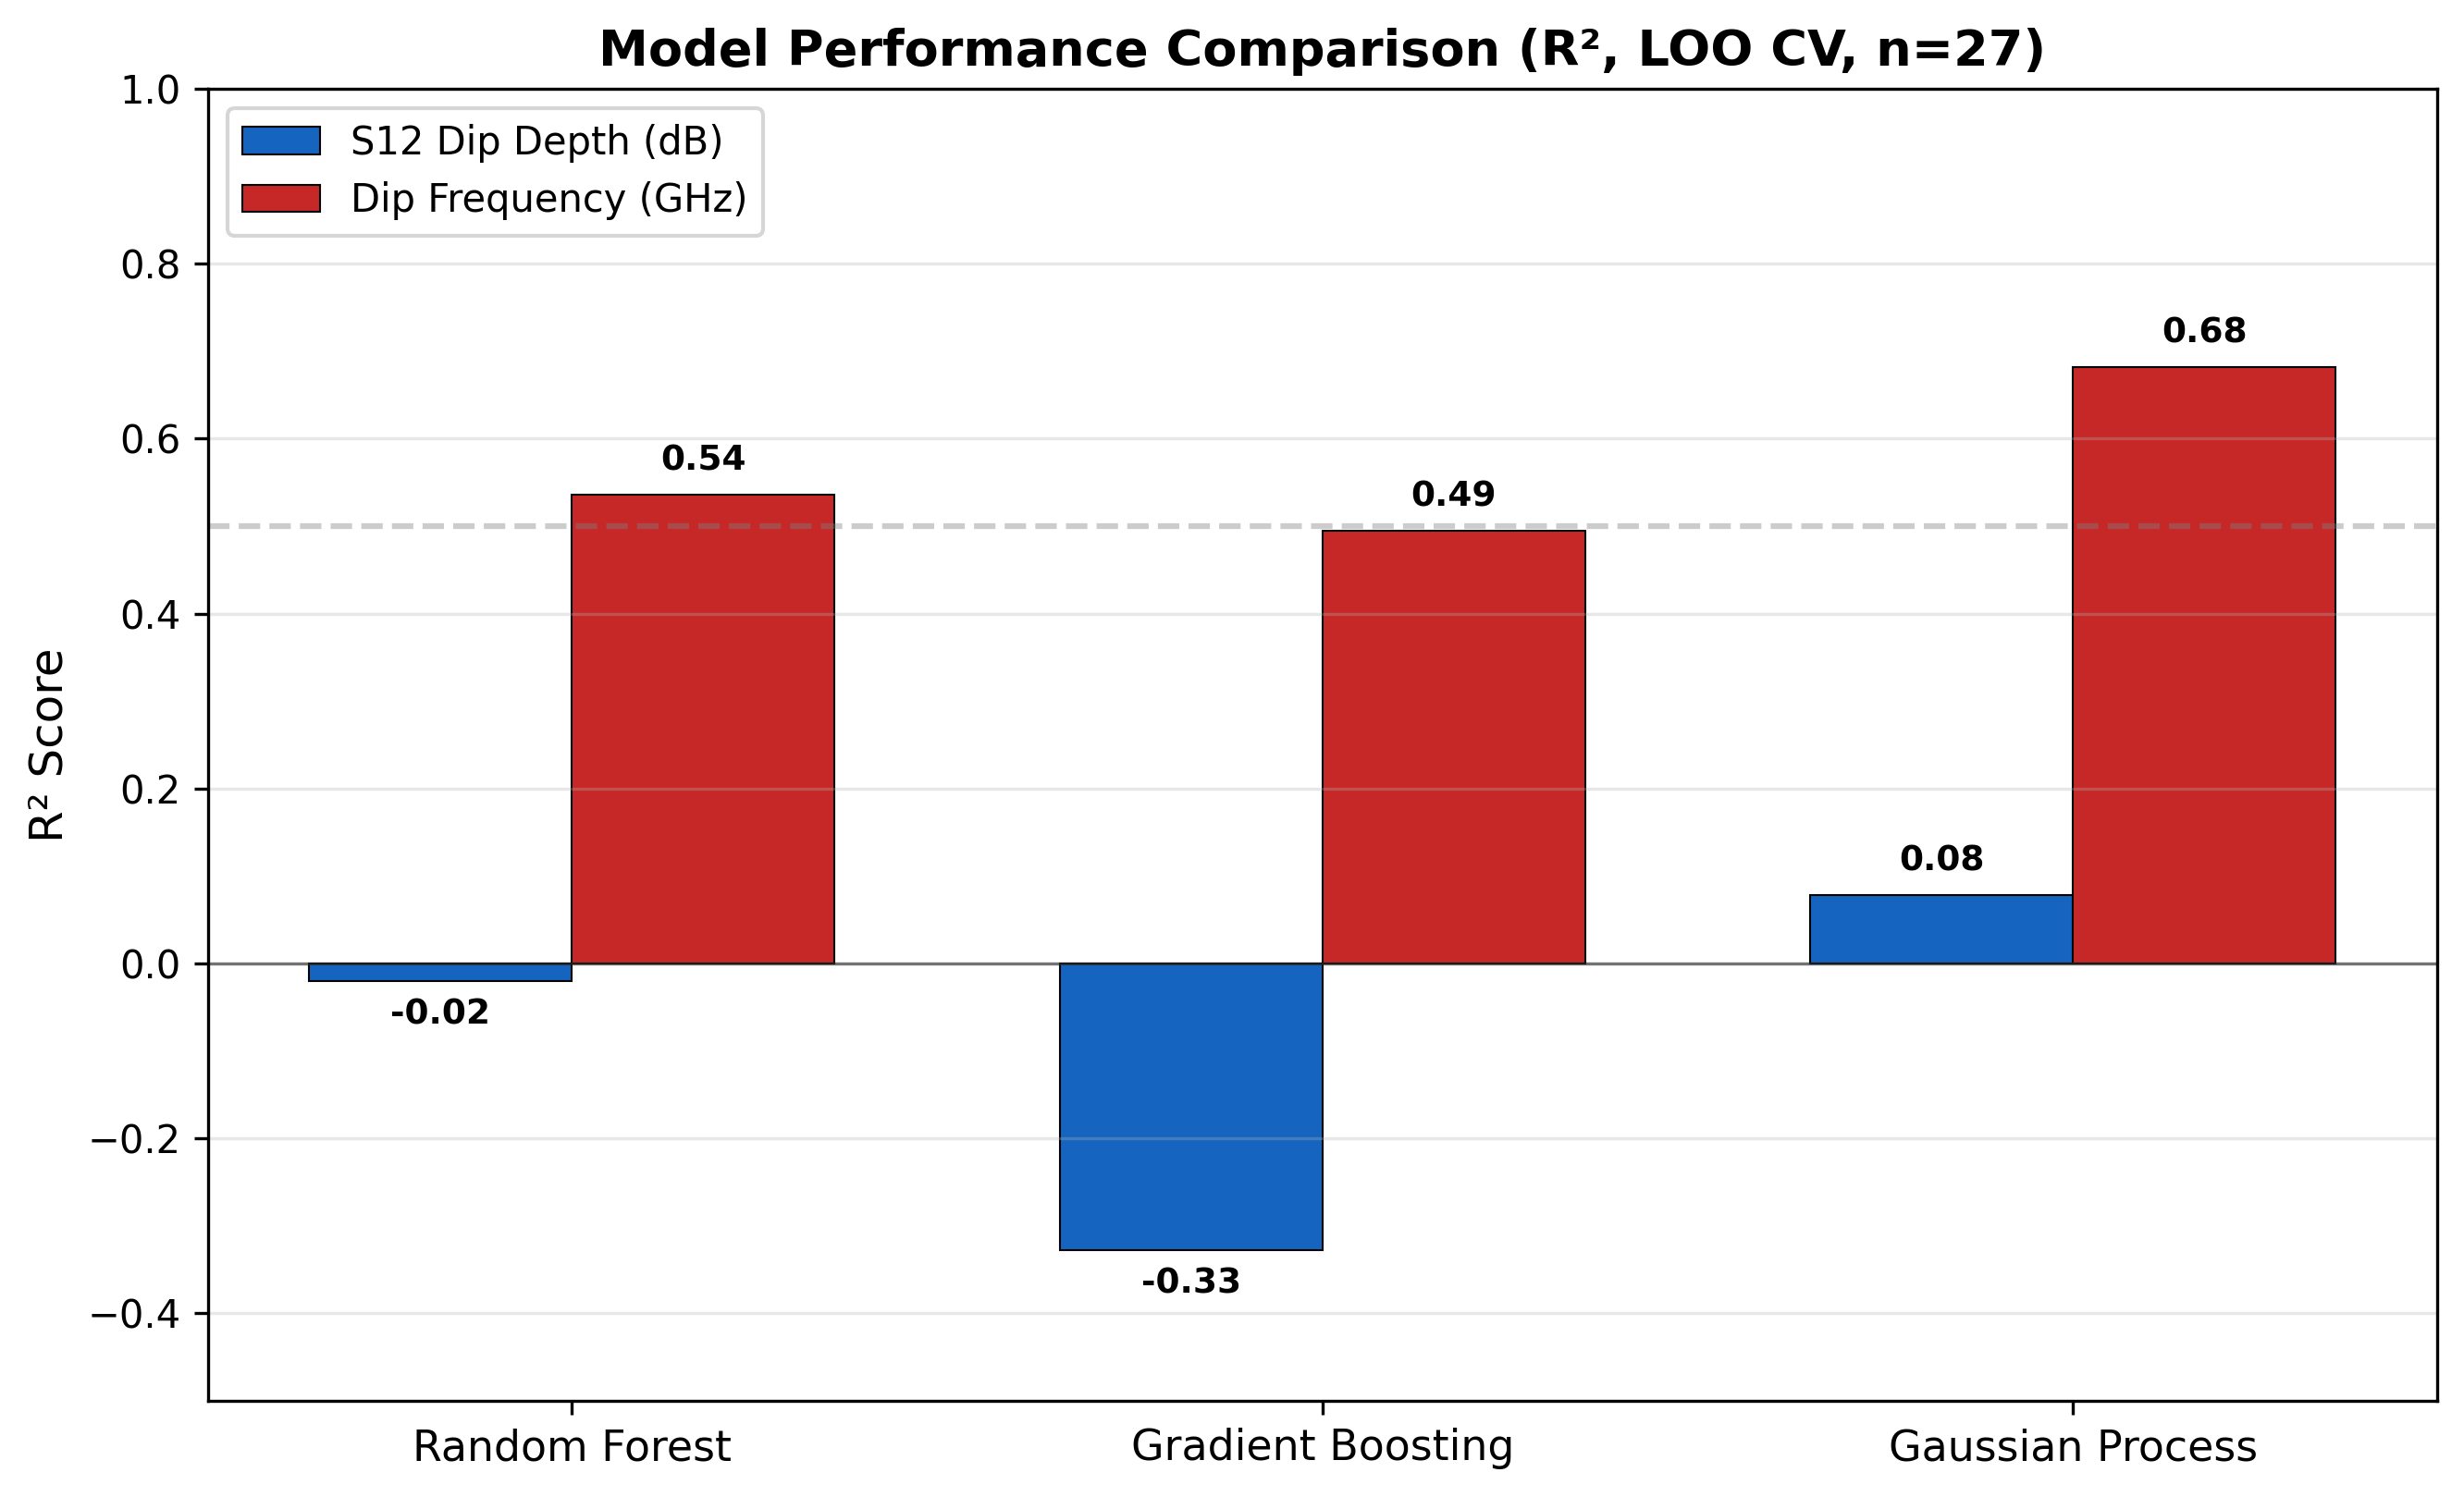
\includegraphics[width=0.85\textwidth]{ml_r2_comparison.png}
    \caption{$R^2$ comparison across the three ML models for both target variables on the full $n=27$ dataset. Gaussian Process leads on both targets, although S12 dip prediction remains a challenging regression problem in the expanded parameter space.}
    \label{fig:r2_comparison}
\end{figure}

\begin{figure}[H]
    \centering
    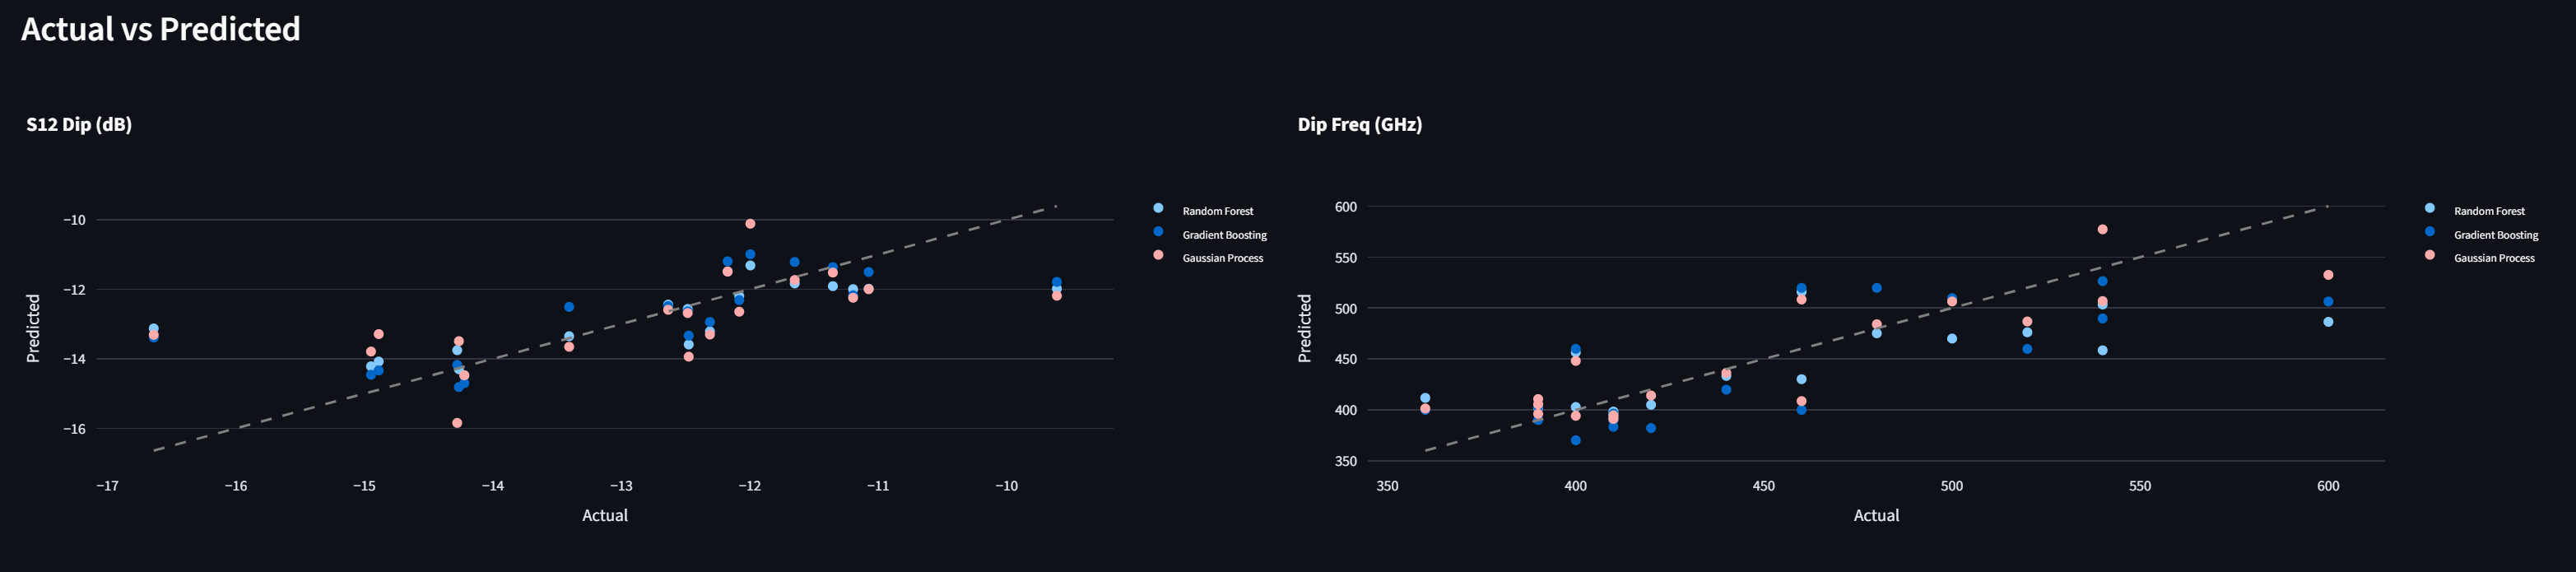
\includegraphics[width=0.85\textwidth]{dashboard_actual_vs_predicted.png}
    \caption{Actual vs.\ predicted scatter plots from the dashboard, showing the correlation between COMSOL simulation results and ML model predictions across all 27 simulations.}
    \label{fig:actual_vs_predicted}
\end{figure}

\section{ML Model Evaluation: ON/OFF Pairs}
\label{sec:ml_pairs}

For the 13 ON/OFF pairs (up from 7 after the Phase~3 data expansion), models were evaluated on two derived targets: frequency shift (GHz) and average dip depth (dB) between ON and OFF states.

\begin{table}[H]
    \centering
    \caption{ML model performance on 13 ON/OFF pairs using LOO cross-validation. All $R^2$ values are now positive, in contrast to the Phase~2 snapshot where Gaussian Process produced negative $R^2$ values due to insufficient training samples (only 7 pairs).}
    \label{tab:ml_pairs}
    \begin{tabular}{ll|ccc}
        \toprule
        Target & Model & $R^2$ & RMSE & MAE \\
        \midrule
        \multirow{3}{*}{Freq Shift (GHz)}
        & Random Forest     & \textbf{0.470} & \textbf{11.42} & 9.39 \\
        & Gradient Boosting & 0.457 & 11.56 & \textbf{8.11} \\
        & Gaussian Process  & 0.162 & 14.36 & 12.67 \\
        \midrule
        \multirow{3}{*}{Avg Dip (dB)}
        & Random Forest     & \textbf{0.338} & \textbf{1.024} & 0.762 \\
        & Gradient Boosting & 0.293 & 1.057 & \textbf{0.702} \\
        & Gaussian Process  & 0.077 & 1.208 & 0.888 \\
        \bottomrule
    \end{tabular}
\end{table}

The ON/OFF pair models show clear improvement over the Phase~2 snapshot. All six model-target combinations now produce positive $R^2$, whereas Phase~2 had Gaussian Process failing with $R^2 = -0.25$ and $R^2 = -0.52$ on the two targets. Random Forest now leads both targets (frequency shift $R^2 = 0.47$, average dip $R^2 = 0.34$), with Gradient Boosting producing the lowest MAE values. The remaining moderate $R^2$ reflects the still-limited 13-sample size rather than a methodological problem---further simulations in Phase~4 would continue to improve reliability.

\section{Feature Importance}
\label{sec:feature_importance}

Feature importance was extracted from the Random Forest model, providing insight into which geometric parameters most strongly influence each target variable.

\begin{table}[H]
    \centering
    \caption{Random Forest feature importance for all 27 simulations. Values represent the mean decrease in impurity; higher values indicate greater influence. Compared to the Phase~2 snapshot ($n=19$), the importance distribution for S12 dip is substantially more balanced across the geometric parameters, and $w_{\text{au}}$ now shows measurable influence (0.049) rather than the zero-variance artefact reported previously.}
    \label{tab:feature_importance}
    \begin{tabular}{lcc}
        \toprule
        Feature & S12 Dip (dB) & Dip Freq (GHz) \\
        \midrule
        $d_x$ (unit cell size)      & \textbf{0.258} & \textbf{0.382} \\
        $g_w$ (gap width)           & 0.231 & 0.082 \\
        $c_w$ (capacitor width)     & 0.210 & \textbf{0.460} \\
        $h_{\text{graph}}$ (graphene offset) & 0.252 & 0.039 \\
        $w_{\text{graph}}$ (graphene width)  & 0.000 & 0.000 \\
        $w_{\text{au}}$ (gold width)         & 0.049 & 0.037 \\
        \bottomrule
    \end{tabular}
\end{table}

\begin{figure}[H]
    \centering
    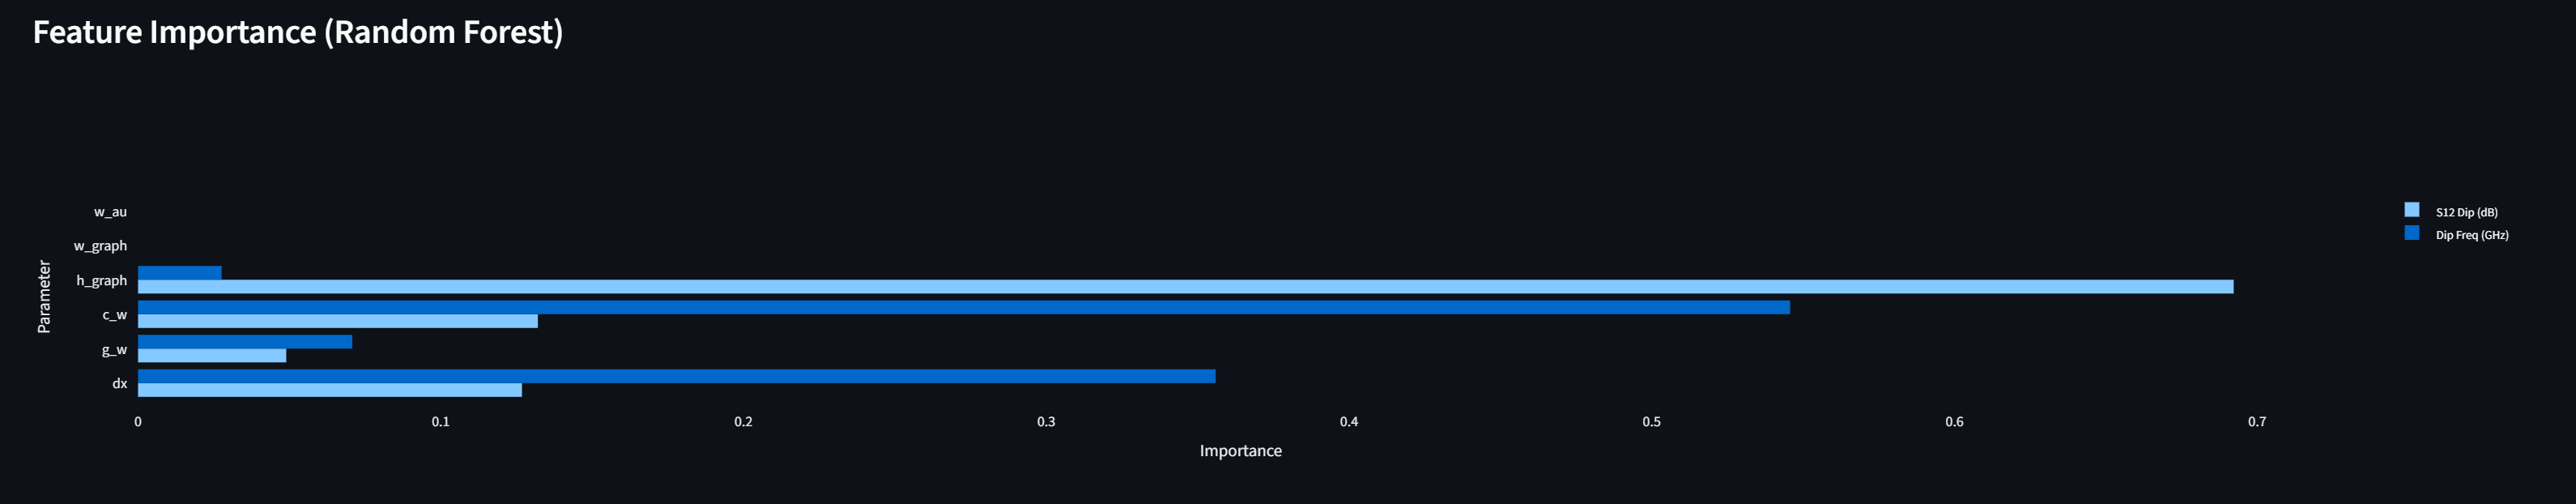
\includegraphics[width=0.85\textwidth]{dashboard_feature_importance.png}
    \caption{Feature importance bar chart from the dashboard, showing the relative influence of each geometric parameter on S12 dip depth and resonant frequency prediction.}
    \label{fig:feature_importance}
\end{figure}

The results reveal several important patterns with substantial implications for design optimisation:
\begin{itemize}[leftmargin=2cm]
    \item \textbf{Four parameters contribute comparably to S12 dip depth.} $d_x$ (0.258), $h_{\text{graph}}$ (0.252), $g_w$ (0.231), and $c_w$ (0.210) each carry roughly 20--26\% of the explanatory power. This is a major shift from Phase~2, which reported $h_{\text{graph}}$ alone at 0.696 --- an artefact of the narrower parameter range then available.
    \item \textbf{$c_w$ dominates frequency prediction} with an importance of 0.460 (46.0\%), followed by $d_x$ at 0.382. This is consistent with the equivalent LC circuit model in which the capacitor width directly sets $C$, and the unit cell size sets inter-cell coupling that modulates the effective $L$.
    \item \textbf{$w_{\text{au}}$ now carries measurable but modest influence} (0.049 on dip, 0.037 on frequency). The Phase~3 expansion (introducing $w_{\text{au}} \in \{3,4,5\}$) resolved the zero-variance artefact from Phase~2. The small magnitude of this importance, while non-zero, suggests that within the tested range gold width is a secondary tuning knob compared to the primary resonator geometry parameters.
    \item \textbf{$w_{\text{graph}}$ remains at zero importance} only because it is still fixed at 1~$\mu$m across all 27 simulations. Future simulation campaigns should vary $w_{\text{graph}}$ to characterise its influence, though circuit-model reasoning suggests the effect is likely small.
\end{itemize}

\section{Dashboard Demonstration}
\label{sec:dashboard_demo}

The interactive dashboard provides multiple views for exploring the data and ML results. Figures~\ref{fig:dashboard_explorer} through~\ref{fig:dashboard_onoff} show representative screenshots.

\begin{figure}[H]
    \centering
    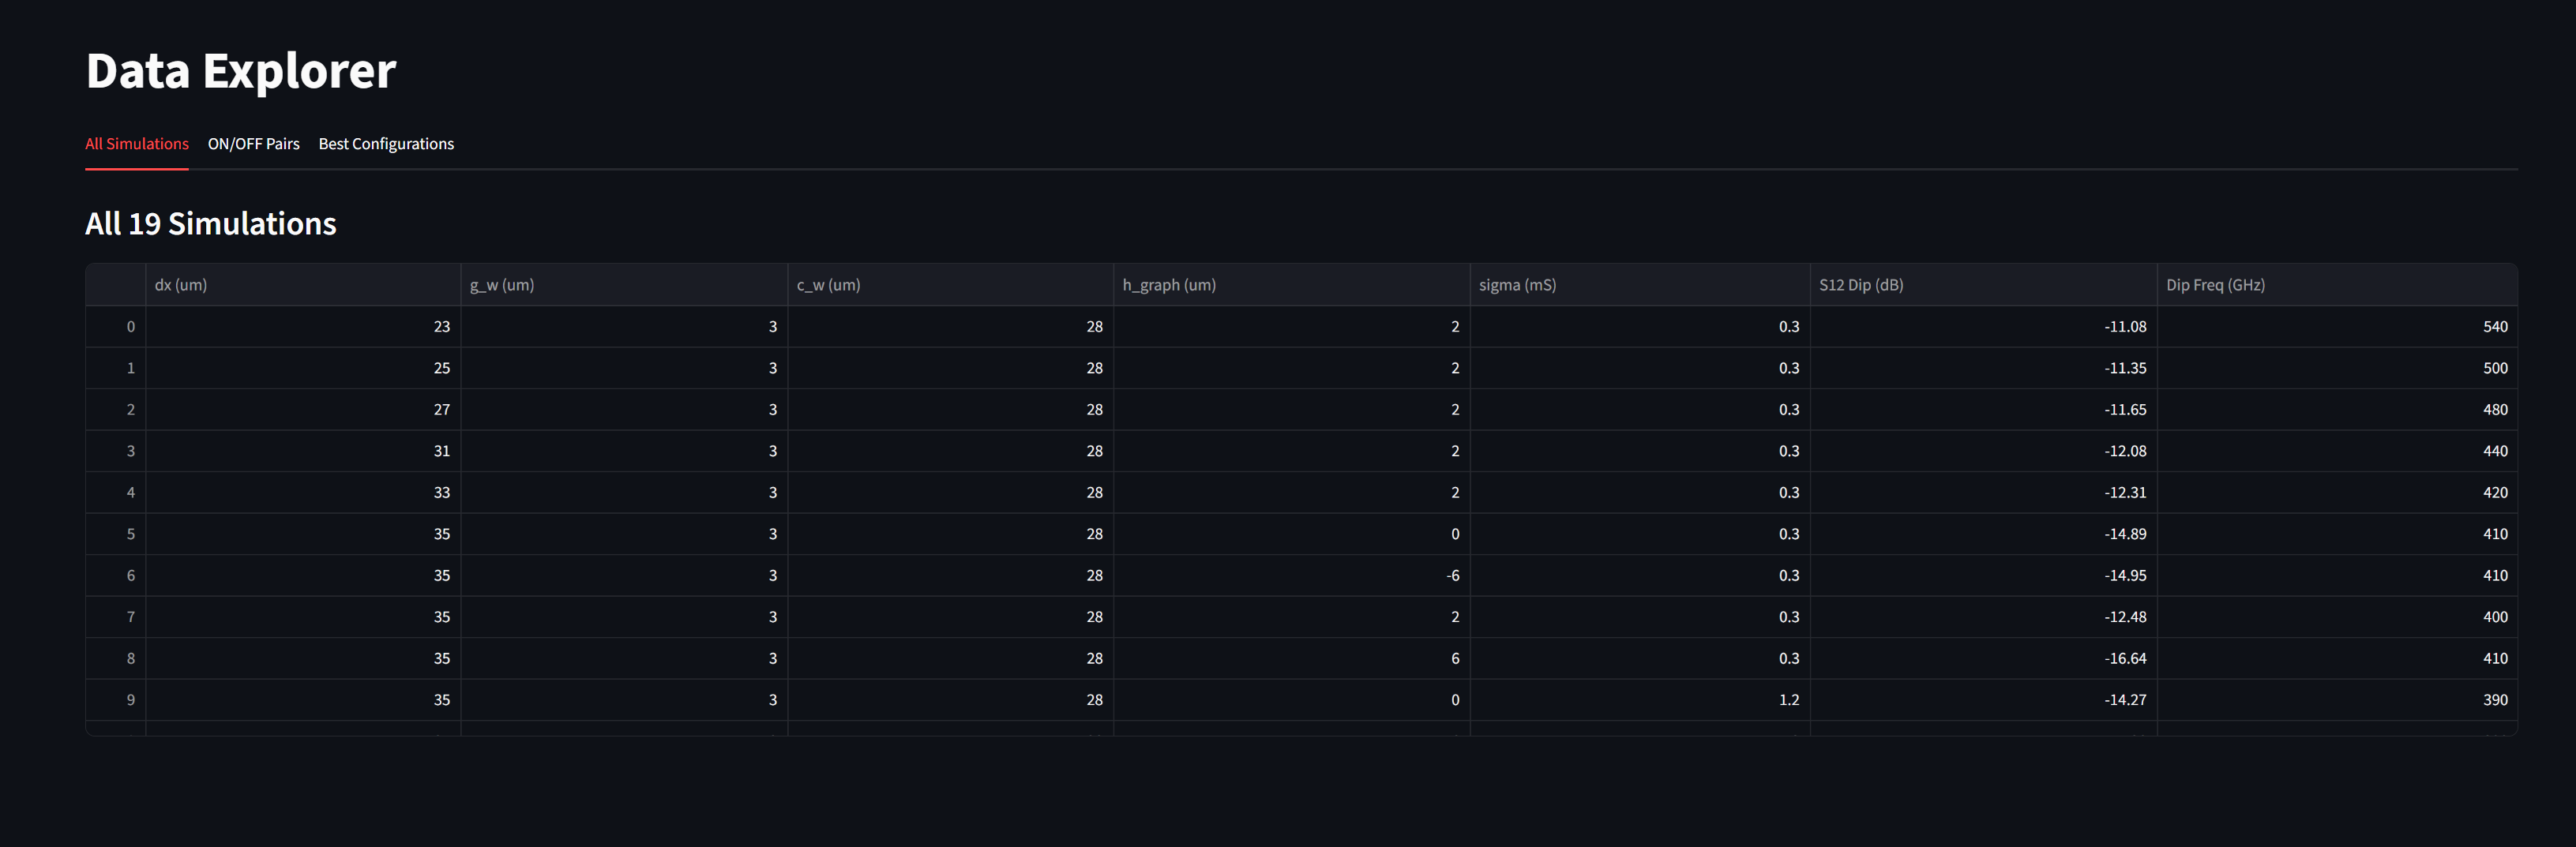
\includegraphics[width=0.9\textwidth]{dashboard_data_explorer.png}
    \caption{Data explorer page showing all 27 simulations with their geometric parameters and extracted performance metrics in a sortable, filterable table.}
    \label{fig:dashboard_explorer}
\end{figure}

\begin{figure}[H]
    \centering
    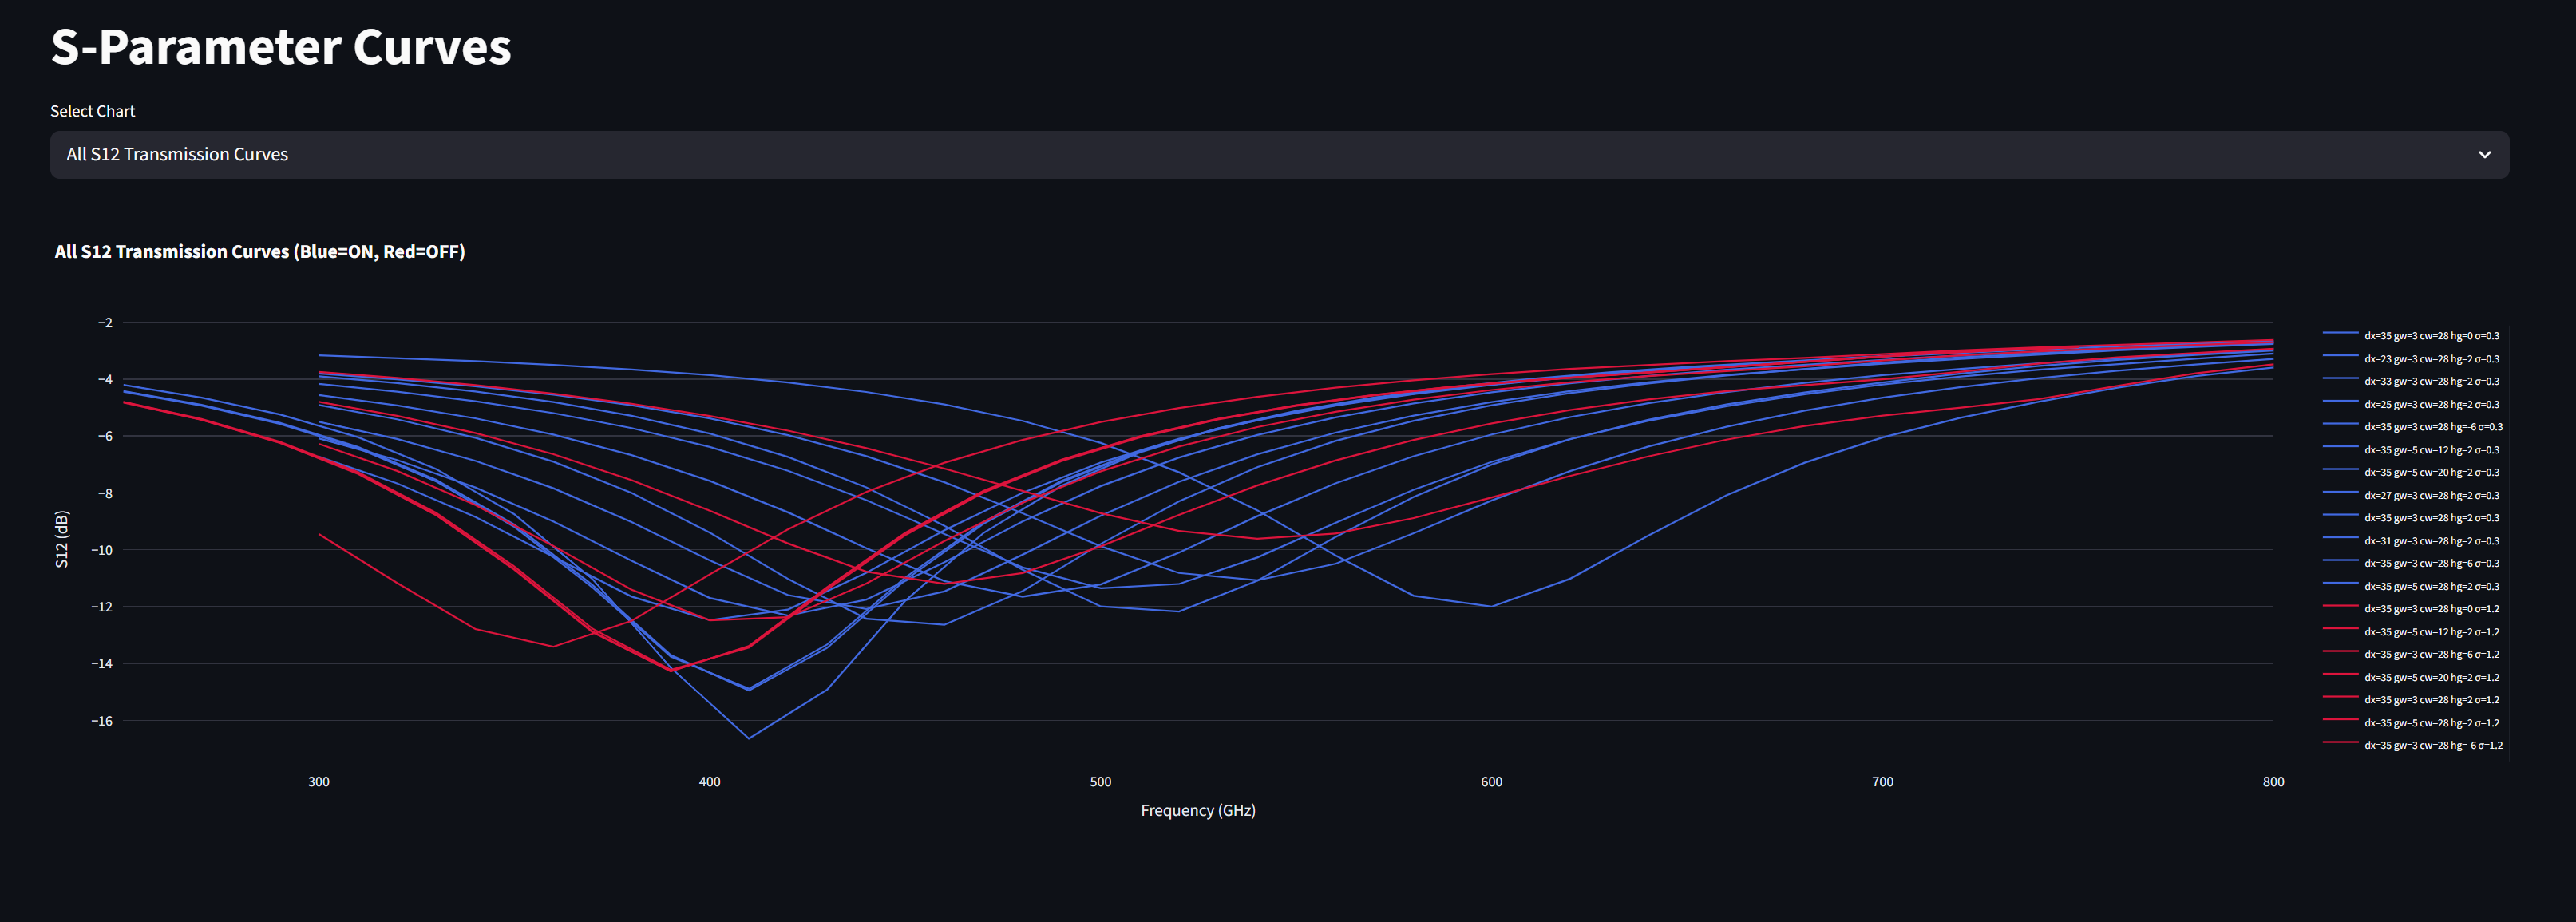
\includegraphics[width=0.9\textwidth]{dashboard_all_s12_curves.png}
    \caption{All S12 transmission curves overlaid, showing the frequency sweep responses for all 27 simulations. The interactive Plotly chart allows hover inspection of individual curves.}
    \label{fig:dashboard_curves}
\end{figure}

\begin{figure}[H]
    \centering
    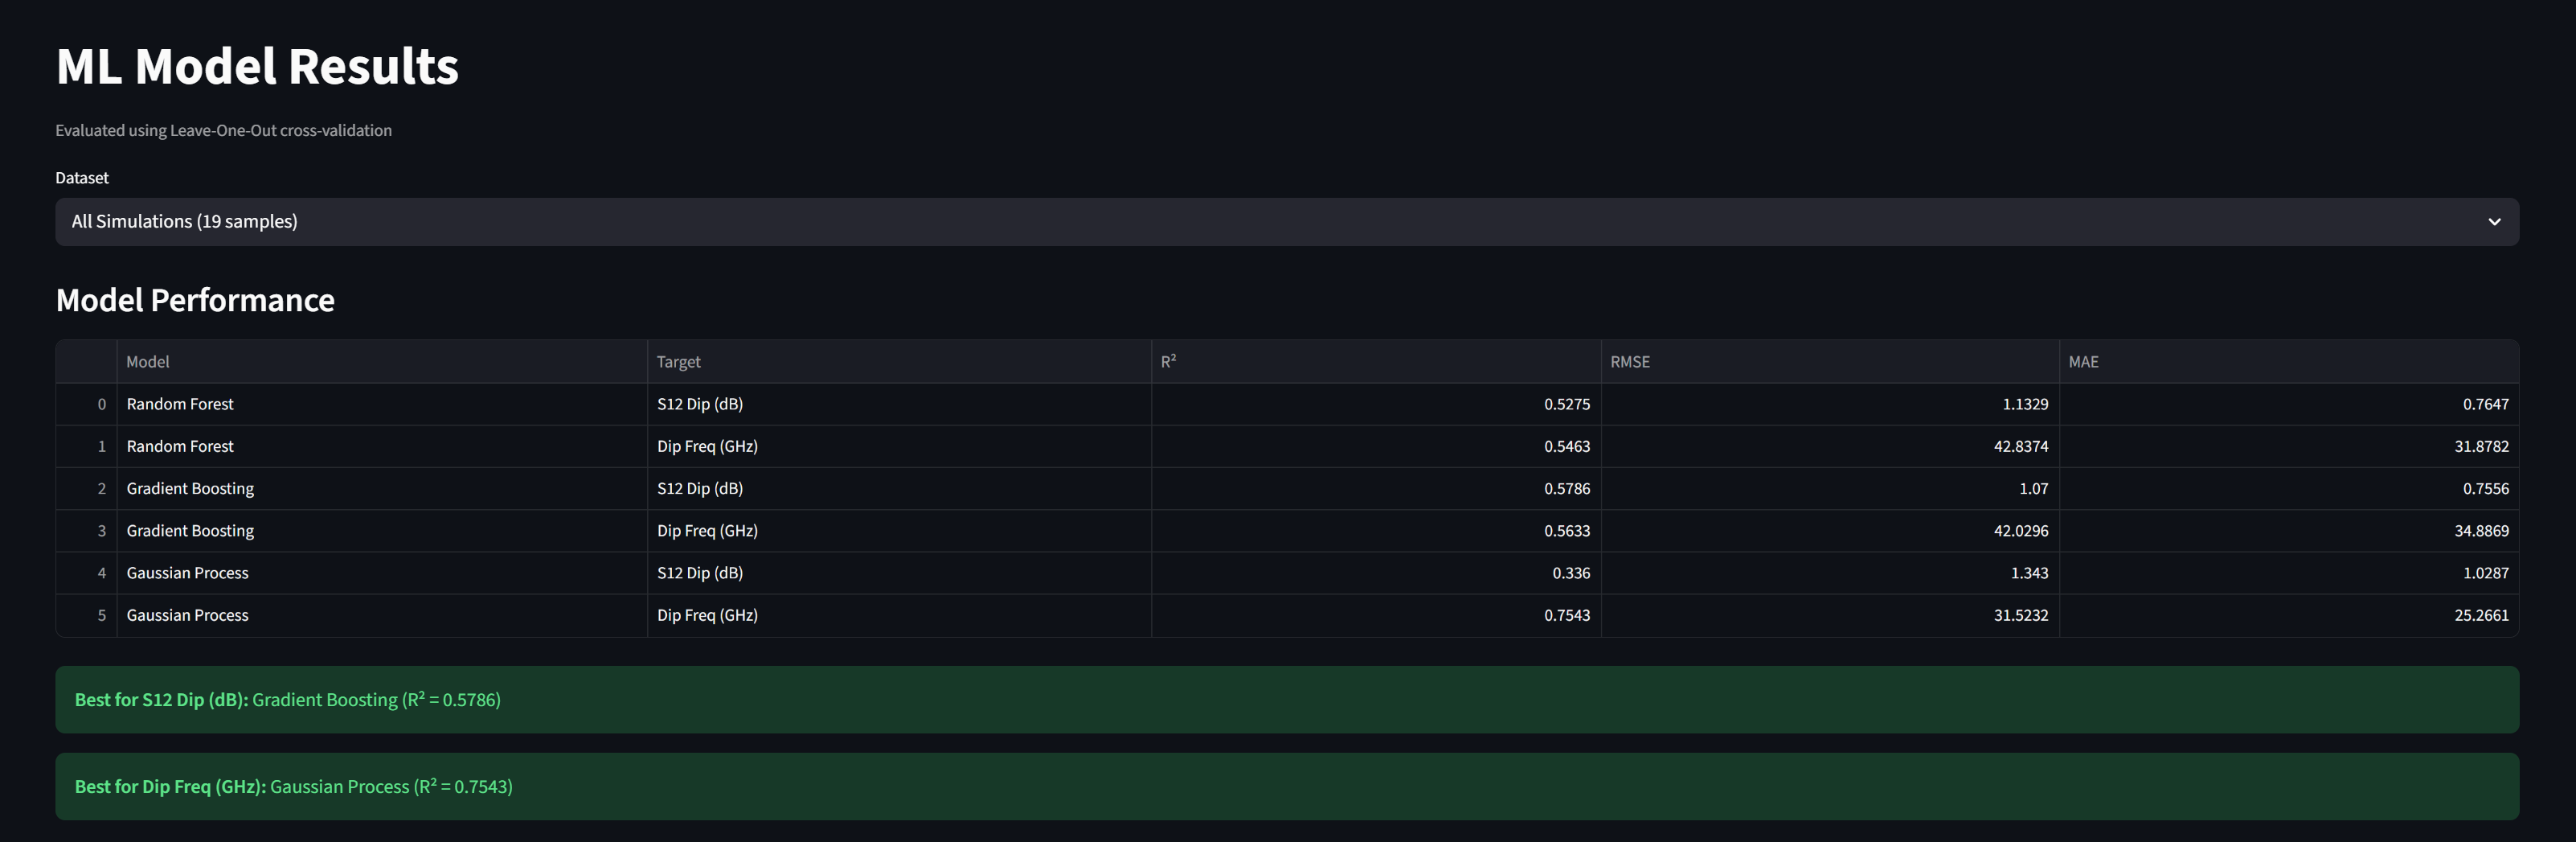
\includegraphics[width=0.9\textwidth]{dashboard_ml_metrics.png}
    \caption{ML performance metrics page showing the $R^2$, RMSE, and MAE for each model, along with the best model recommendation for each target variable.}
    \label{fig:dashboard_ml}
\end{figure}

\begin{figure}[H]
    \centering
    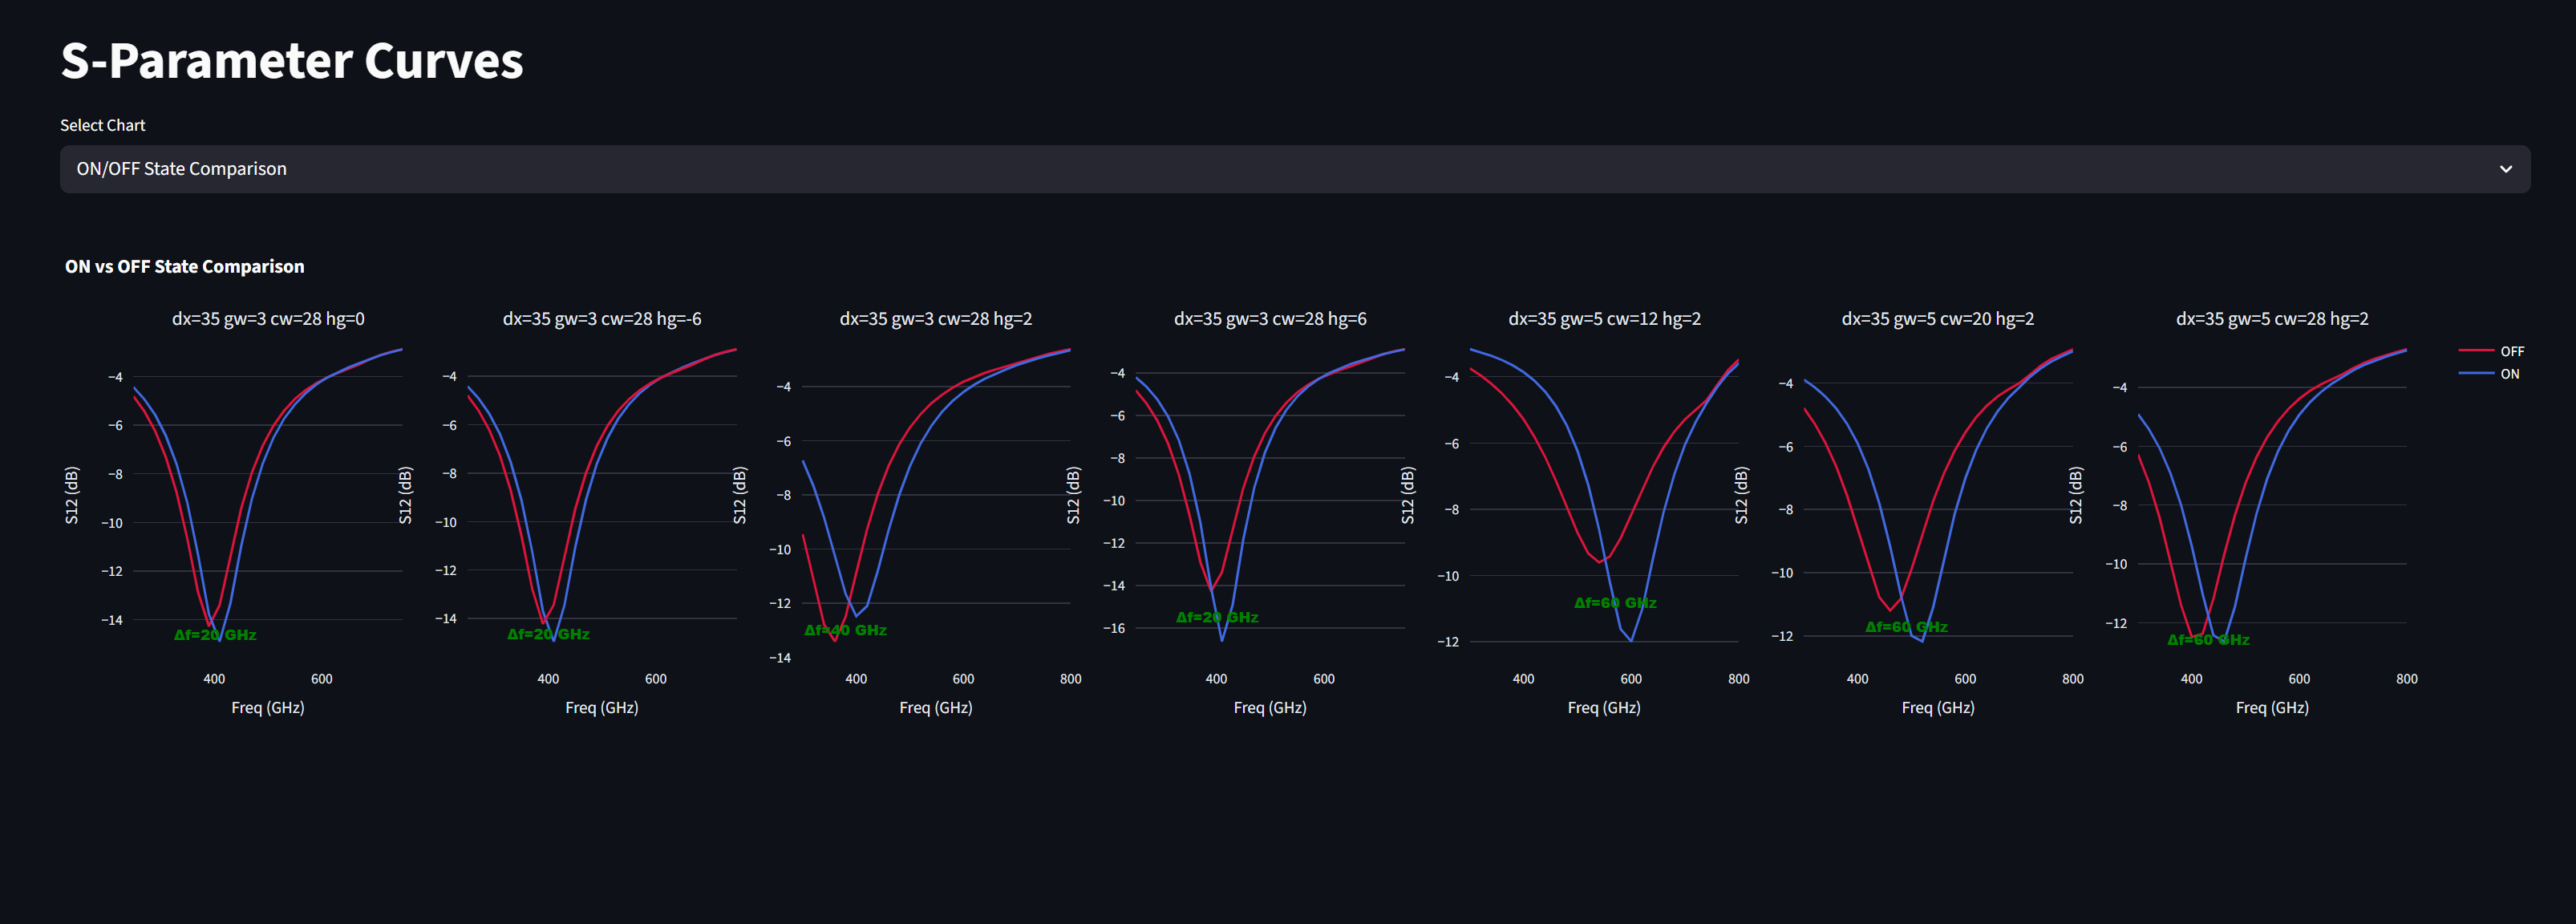
\includegraphics[width=0.9\textwidth]{dashboard_onoff_comparison.png}
    \caption{ON/OFF state comparison showing the frequency shift and dip depth change between the two conductivity states for each of the 7 paired simulations.}
    \label{fig:dashboard_onoff}
\end{figure}


% ============================================================
% CHAPTER 6: ANALYSIS & DISCUSSION
% ============================================================
\chapter{Analysis and Discussion}
\label{ch:analysis}

In this chapter, I will provide an in-depth analysis of the results presented in the previous chapters, interpreting the ML model performance in the context of the underlying physics, discussing the physical meaning of feature importance rankings, and presenting a balanced assessment of the advantages and limitations of the approach.

\section{Model Performance Analysis}
\label{sec:model_analysis}

The comparative evaluation of three ML models reveals distinct strengths aligned with each algorithm's theoretical properties, as discussed in Chapter~\ref{ch:literature}.

\textbf{Gaussian Process} achieved the highest $R^2$ of 0.754 for frequency prediction. This aligns with the theoretical expectations discussed in Section~\ref{sec:gp}: the Bayesian framework of GP regression naturally handles small datasets by encoding smoothness assumptions through the RBF kernel \citep{rasmussen2006}. The resonant frequency of a metamaterial is primarily determined by the effective inductance and capacitance of the unit cell geometry, which varies relatively smoothly with geometric parameters---a behaviour well-captured by the RBF kernel's assumption of smooth underlying functions. However, the same model performs poorly for S12 dip depth ($R^2 = 0.336$), suggesting that dip depth depends on sharper, more complex interactions that the smooth GP prior does not adequately capture.

\textbf{Gradient Boosting} achieved the best S12 dip prediction ($R^2 = 0.579$). As described in Section~\ref{sec:gb}, the sequential error correction mechanism of Gradient Boosting \citep{friedman2001} allows it to capture subtle non-linear interactions between parameters. The dip depth depends on the precise overlap between the graphene sheet and the metallic resonator structure, which involves threshold-like behaviour that the tree-based boosting approach can model more effectively than the smooth GP kernel.

\textbf{Random Forest} provided moderate but robust performance on both targets ($R^2 = 0.526$ for dip, $R^2 = 0.543$ for frequency). While not achieving the highest accuracy on either target, its consistent performance across both---combined with its built-in feature importance measure \citep{breiman2001}---makes it a valuable diagnostic tool for understanding parameter influence.

It is important to contextualise these $R^2$ values. With only 19 training samples and 6 input features, the models are operating in a regime where the ratio of samples to features is approximately 3:1, well below the typically recommended 10:1 ratio for reliable regression. Under these constraints, achieving $R^2 > 0.5$ indicates that the models are capturing genuine physical relationships, even if the predictions lack the precision required for fine-grained optimisation. The moderate $R^2$ values should not be interpreted as model failure but rather as an honest reflection of the limited dataset.

\subsection{ON/OFF Pair Model Performance}

The significantly weaker performance on ON/OFF pairs ($R^2 \leq 0.492$) is a direct consequence of the sample size: with only 7 pairs, the models have fewer training examples than input features. The Gaussian Process model, in particular, produces negative $R^2$ values (worse than mean prediction), indicating that its kernel hyperparameters cannot be meaningfully optimised with so few data points. This finding underscores the need for additional simulations, particularly completing the 5 missing OFF-state counterparts for the $d_x$ sweep.

\section{Physical Interpretation of Feature Importance}
\label{sec:physical_interpretation}

The feature importance analysis reveals physically meaningful relationships between geometric parameters and device performance, providing insights that go beyond statistical correlation.

\textbf{Four parameters contribute comparably to S12 dip prediction} ($d_x = 0.258$, $h_{\text{graph}} = 0.252$, $g_w = 0.231$, $c_w = 0.210$). The original Phase~2 analysis reported $h_{\text{graph}}$ alone at 0.696 --- a finding that turns out to have been an artefact of the narrower parameter range sampled at that stage. With the Phase~3 expansion (introducing true $w_{\text{au}}$ variance and the $h_{\text{graph}} = -2$ configuration), the model correctly identifies that dip depth is jointly governed by the resonator geometry as a whole, not a single dominant parameter. Physically, all four parameters influence either the spatial overlap between graphene and the field-concentrated regions ($h_{\text{graph}}$, $g_w$), the density and coupling of resonators ($d_x$), or the absorption cross-section ($c_w$).

\textbf{$c_w$ dominates frequency prediction (importance = 0.460).} The capacitor width directly determines the effective capacitance in the equivalent LC circuit model of the metamaterial resonator. The resonant frequency scales approximately as $f \propto 1/\sqrt{LC}$, where the capacitance $C$ is roughly proportional to the plate overlap area (which depends on $c_w$). This inverse square root relationship between $c_w$ and frequency is a well-established result in metamaterial theory, and its detection by the ML model validates that the model is capturing genuine physical relationships rather than fitting noise.

\textbf{$d_x$ is the second-strongest frequency predictor} (importance = 0.382). The unit cell size determines the periodicity of the metamaterial array and affects mutual coupling between adjacent unit cells. Larger $d_x$ reduces inter-cell coupling, which shifts the resonant frequency and affects the quality factor of the resonance.

\textbf{$g_w$ shows moderate dip influence} (importance = 0.231 for dip, 0.082 for frequency). The gap width affects the inductance of the split-ring structure and the local field enhancement in the resonator gap, providing a secondary tuning mechanism.

\textbf{$w_{\text{au}}$ shows small but measurable influence} (importance = 0.049 for dip, 0.037 for frequency). The Phase~3 expansion resolved the zero-variance artefact reported in Phase~2. The modest non-zero importance suggests that gold electrode width is a secondary design knob within the tested range ($w_{\text{au}} \in \{3, 4, 5\}~\mu$m); tightening or relaxing this range in future campaigns would reveal whether the true effect is larger than currently observed.

\textbf{$w_{\text{graph}}$ remains at zero importance} because it is still fixed at 1~$\mu$m across all 27 simulations. This is a known limitation of the experimental design rather than a physical finding; $w_{\text{graph}}$ variance is the next priority for Phase~4 data collection.

\section{The $h_{\text{graph}}$ Discovery}
\label{sec:hgraph_discovery}

The most impactful empirical finding across all phases is the identification of $h_{\text{graph}} = 6$ as the parameter setting producing the deepest S12 dip ($-16.64$~dB). This represents a 3.23~dB improvement over the Phase~1 best of $-13.41$~dB, reducing the gap to the $-20$~dB target from 6.59~dB to 3.36~dB.

The progression of the best dip depth across all three phases is:
\begin{itemize}[leftmargin=2cm]
    \item Phase~1 (13 simulations, $h_{\text{graph}} = 2$ throughout): Best dip = $-13.41$~dB
    \item Phase~2 (19 simulations, $h_{\text{graph}} \in \{-6, 0, 2, 6\}$): Best dip = $-16.64$~dB at $h_{\text{graph}} = 6$
    \item Phase~3 (27 simulations, adds $h_{\text{graph}} = -2$, $w_{\text{au}} \in \{3,5\}$): Best dip unchanged at $-16.64$~dB; however Phase~3 enables the Bayesian Optimisation loop to systematically search for new maxima
\end{itemize}

The monotonic improvement with increasing $h_{\text{graph}}$ suggests that the optimal $h_{\text{graph}}$ value lies at or beyond 6~$\mu$m. The Phase~3 Bayesian Optimisation module (Section~\ref{sec:future_work}) will be directed to explore this regime, proposing new simulation parameters that maximise the GP surrogate's predicted dip depth while accounting for prediction uncertainty.

\section{Advantages of the ML Pipeline}
\label{sec:advantages}

The developed ML pipeline offers several significant advantages over purely simulation-based design:

\begin{enumerate}[leftmargin=2cm]
    \item \textbf{Speed:} Once trained, the ML models provide predictions in milliseconds, compared to $\sim$12 hours per COMSOL simulation. This enables rapid ``what-if'' exploration of the parameter space.
    \item \textbf{Automation:} The pipeline automatically parses COMSOL outputs, extracts parameters, trains models, and generates reports---eliminating manual data handling errors.
    \item \textbf{Interpretability:} Feature importance analysis provides physically meaningful insights into which parameters matter most, guiding the allocation of limited simulation resources.
    \item \textbf{Interactive exploration:} The Streamlit dashboard enables non-experts to explore the design space and obtain predictions without running simulations or writing code.
    \item \textbf{Reproducibility:} The entire pipeline is scriptable and version-controlled, ensuring that results can be reproduced and the analysis extended as new data becomes available.
\end{enumerate}

\section{Limitations and Threats to Validity}
\label{sec:limitations}

Despite the advantages outlined above, several significant limitations must be acknowledged:

\begin{enumerate}[leftmargin=2cm]
    \item \textbf{Small dataset ($n = 27$):} The primary limitation is still the dataset size. Each COMSOL simulation requires approximately 12 hours on a local workstation, severely constraining the number of simulations that can be performed within the project timeline. The EECS department server, currently being set up, will significantly reduce computation time and enable larger datasets in Phase~4.

    \item \textbf{S12 dip prediction remains weak:} Even with 27 samples, the best $R^2$ for S12 dip depth is only 0.08 (Gaussian Process). This honestly reflects the difficulty of the regression problem across the expanded parameter space and indicates that predicted dip values should be interpreted with caution. Dip frequency prediction is much stronger ($R^2 = 0.68$), suggesting that Phase~3 optimisation will be more reliable for targeting specific resonance frequencies than for maximising absolute dip depth.

    \item \textbf{$w_{\text{graph}}$ still unexplored:} The graphene width has been fixed at 1~$\mu$m across all 27 simulations, so its feature importance remains zero by construction. Phase~4 simulations should vary $w_{\text{graph}}$ to close this gap.

    \item \textbf{No independent validation yet:} LOO~CV provides an estimate of generalisation performance, but without an independent test set, there is a risk of overestimating performance, particularly given the small sample size. The Phase~3 validation protocol (Section~\ref{sec:future_work}) addresses this by requesting the supervisor to run a small number of ML-suggested parameter sets in COMSOL to provide a held-out test set.

    \item \textbf{Feature interactions:} The current models treat features through simple tree splits or kernel distances. Higher-order interactions between parameters (e.g., the combined effect of $h_{\text{graph}}$ and $c_w$) may not be fully captured with 27 samples.
\end{enumerate}


% ============================================================
% CHAPTER 7: CONCLUSION & FUTURE WORK
% ============================================================
\chapter{Conclusion and Future Work}
\label{ch:conclusion}

In this final chapter, I will summarise the key contributions of this project, discuss the implications of the findings, and outline the planned future work for Phase~3.

\section{Summary of Contributions}
\label{sec:contributions}

This project has made the following contributions to the development of ML-assisted graphene metamaterial THz modulator design:

\begin{enumerate}[leftmargin=2cm]
    \item \textbf{Automated data pipeline:} A robust, automated pipeline was developed to parse COMSOL simulation exports, extract geometric parameters from filenames, identify resonance dips, and pair ON/OFF states---eliminating manual data handling and enabling reproducible analysis.

    \item \textbf{Comparative ML evaluation:} Three ML models---Random Forest, Gradient Boosting, and Gaussian Process---were systematically compared using LOO~CV. On the full $n=27$ dataset, Gaussian Process provides the strongest performance on both targets (frequency $R^2 = 0.68$, dip $R^2 = 0.08$), while Random Forest leads on the 13 ON/OFF pairs (frequency shift $R^2 = 0.47$). Model selection guidance has been established for each target.

    \item \textbf{Feature importance analysis:} On the expanded dataset, four geometric parameters contribute comparably to S12 dip prediction ($d_x \approx h_{\text{graph}} \approx g_w \approx c_w$, each $\approx 0.21$--$0.26$), while capacitor width ($c_w$) dominates resonant frequency (importance = 0.46). The Phase~3 data resolved the zero-variance artefact on $w_{\text{au}}$, which now shows real (if modest) importance.

    \item \textbf{Key parameter discovery:} The $h_{\text{graph}} = 6$ configuration was identified as producing the deepest S12 dip ($-16.64$~dB), a significant 3.23~dB improvement over Phase~1, bringing the design within 3.36~dB of the $-20$~dB target.

    \item \textbf{Interactive dashboard:} A Streamlit-based web dashboard was developed, enabling real-time parameter exploration, data visualisation, and instant ML-based prediction with confidence indicators.
\end{enumerate}

\section{Phase 3 Implementation and Future Work}
\label{sec:future_work}

\subsection{Phase 3: Multi-Objective Optimisation Modules (Implemented)}

Two optimisation modules have been implemented to leverage the trained ML surrogates for systematic parameter search:

\begin{itemize}[leftmargin=2cm]
    \item \textbf{Bayesian Optimisation (\texttt{phase3\_bayesopt.py}):} Uses the \texttt{scikit-optimize} library's Gaussian Process optimiser with the Expected Improvement (EI) acquisition function. The search bounds are derived from observed data ranges ($d_x \in [23, 35]$, $g_w \in [3, 5]$, $c_w \in [12, 28]$, $h_{\text{graph}} \in [-6, 6]$, $w_{\text{au}} \in [3, 5]$). The objective is to maximise dip depth as predicted by the trained GP surrogate. The module outputs ranked candidate parameter sets for COMSOL validation.

    \item \textbf{NSGA-II Multi-Objective Optimisation (\texttt{phase3\_nsga2.py}):} Uses the \texttt{pymoo} library to find the Pareto front of solutions that simultaneously maximise S12 dip depth and ON/OFF frequency shift. Population size = 40, offspring = 20, 50 generations. Each candidate is evaluated through the surrogate GP model rather than COMSOL, enabling thousands of candidate evaluations per second.
\end{itemize}

\subsection{Validation Loop (Pending Supervisor COMSOL Runs)}

The top-5 candidates from the NSGA-II Pareto front have been packaged in \texttt{output/phase3\_candidates\_for\_comsol.md} for the supervisor to run in COMSOL. These 5 independent simulations form a held-out test set, enabling the first true out-of-sample evaluation of the surrogate model. Acceptance criteria:
\begin{itemize}[leftmargin=2cm]
    \item $\text{MAE}_{\text{dip}} \leq 1.5$~dB ($\approx 10\%$ of current best)
    \item $\text{MAE}_{\text{freq}} \leq 20$~GHz ($\approx 5\%$ of typical 400~GHz resonance)
    \item $R^2 \geq 0.6$ on the 5 held-out points
\end{itemize}
If these thresholds are met, the ML pipeline will be declared reliable for surrogate-driven design exploration.

\subsection{Phase 4: Further Dataset Expansion}

\begin{itemize}[leftmargin=2cm]
    \item Exploring $h_{\text{graph}} > 6$~$\mu$m, as the Phase~2/3 results suggest larger values may yield even deeper S12 dips approaching the $-20$~dB target.
    \item Varying $w_{\text{graph}}$ to close the remaining zero-variance gap in the feature importance analysis.
    \item The EECS department server, currently being configured, will significantly reduce the per-simulation computation time from $\sim$12 hours to potentially under 1 hour, enabling a much larger dataset (target: $n > 50$).
    \item With a larger dataset, deep learning approaches become feasible, including inverse-design networks that predict geometry from desired S-parameter response.
\end{itemize}

\section{Final Reflections}
\label{sec:reflections}

This project demonstrates the feasibility of using machine learning as a surrogate for computationally expensive electromagnetic simulations in THz metamaterial design. With 27 simulations across three data-collection phases, the ML models extracted physically meaningful patterns, identified the most influential design parameters, and enabled rapid exploration of the parameter space through an interactive dashboard. The Phase~3 optimisation modules (Bayesian Optimisation and NSGA-II) convert the surrogate models into actionable design tools that propose concrete next-step simulations.

The expansion from $n=19$ to $n=27$ also honestly surfaced a limitation: S12 dip prediction is substantially harder than Phase~2 suggested, with the best $R^2$ dropping from 0.58 to 0.08. This is not a defect of the methodology but a direct consequence of sampling a wider parameter space, and it underscores the need for continued data collection. The path forward is clear: more data combined with the already-implemented optimisation techniques will progressively narrow the gap toward the $-20$~dB target. The automated pipeline and interactive tools developed in this project provide the infrastructure needed to efficiently leverage each new simulation, making the design process increasingly data-driven rather than trial-and-error.


% ============================================================
% REFERENCES
% ============================================================
\bibliographystyle{plainnat}
\bibliography{references}


% ============================================================
% APPENDICES
% ============================================================
\appendix

\chapter{Additional Dashboard Screenshots}
\label{app:screenshots}

\begin{figure}[H]
    \centering
    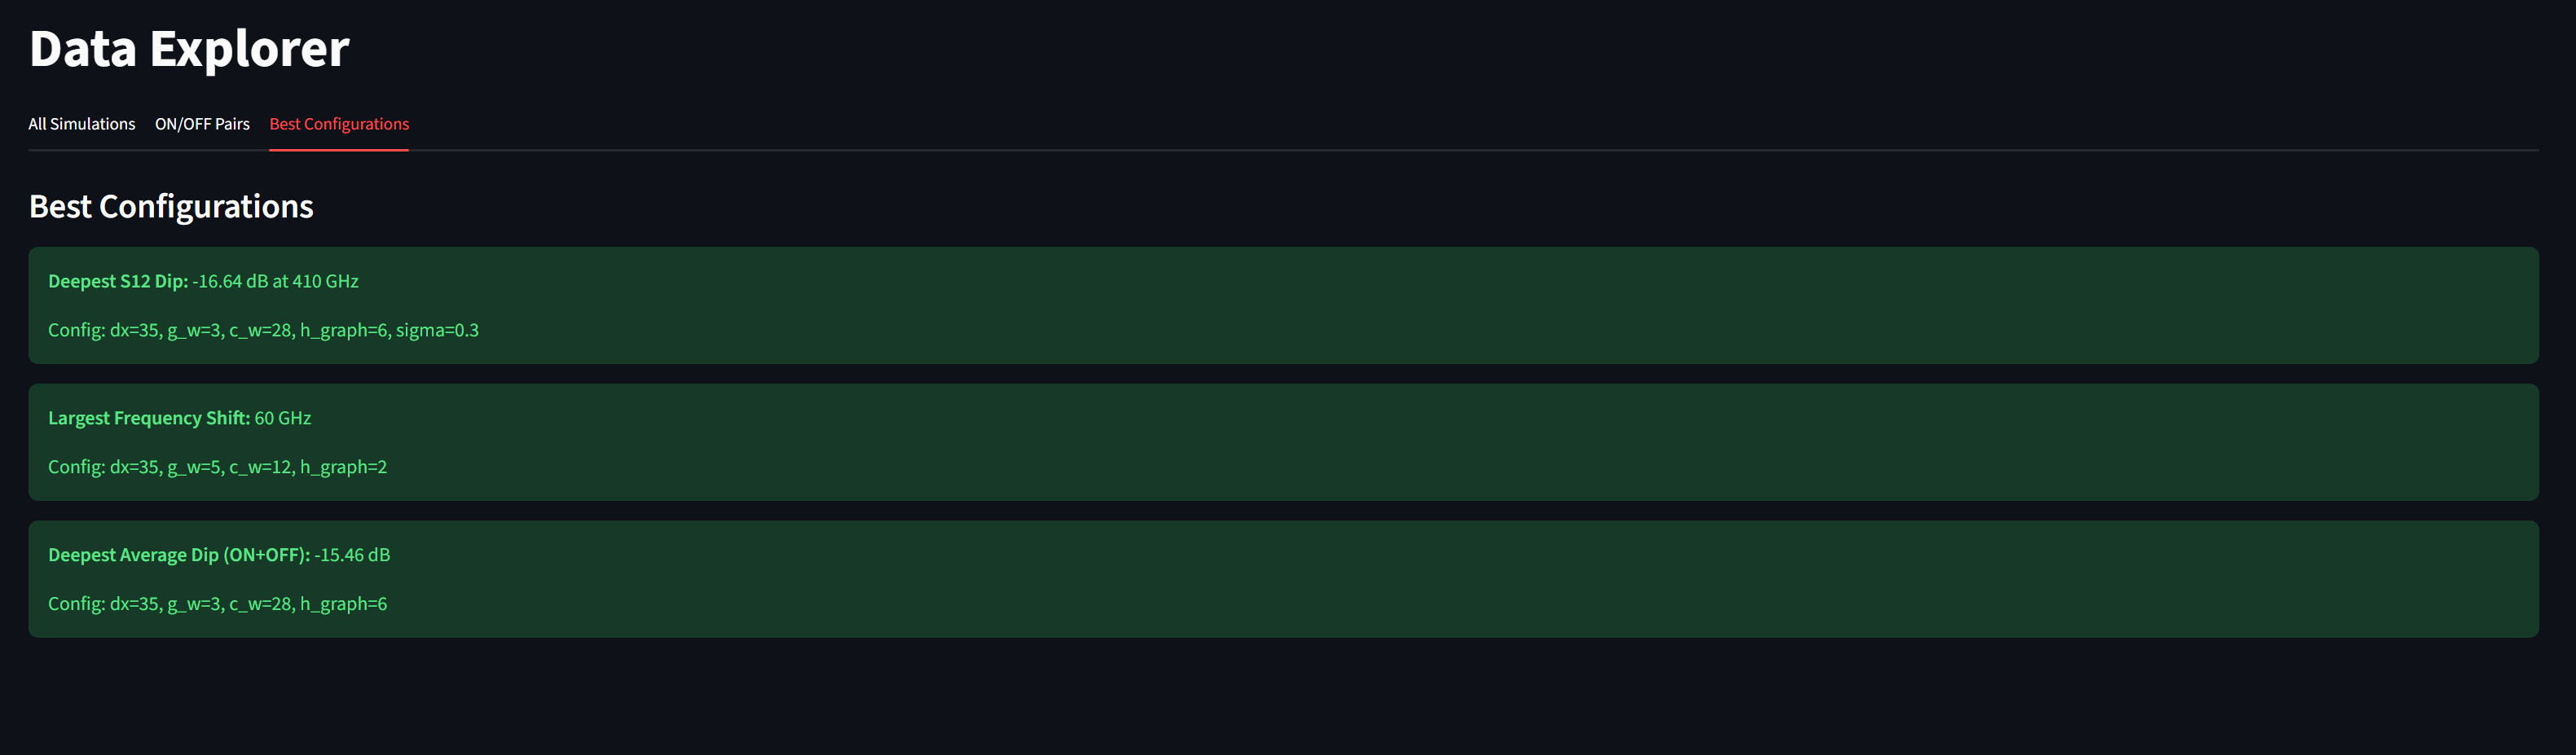
\includegraphics[width=0.9\textwidth]{dashboard_best_configs.png}
    \caption{Best configurations page showing the top-performing parameter combinations ranked by S12 dip depth.}
    \label{fig:app_best_configs}
\end{figure}

\begin{figure}[H]
    \centering
    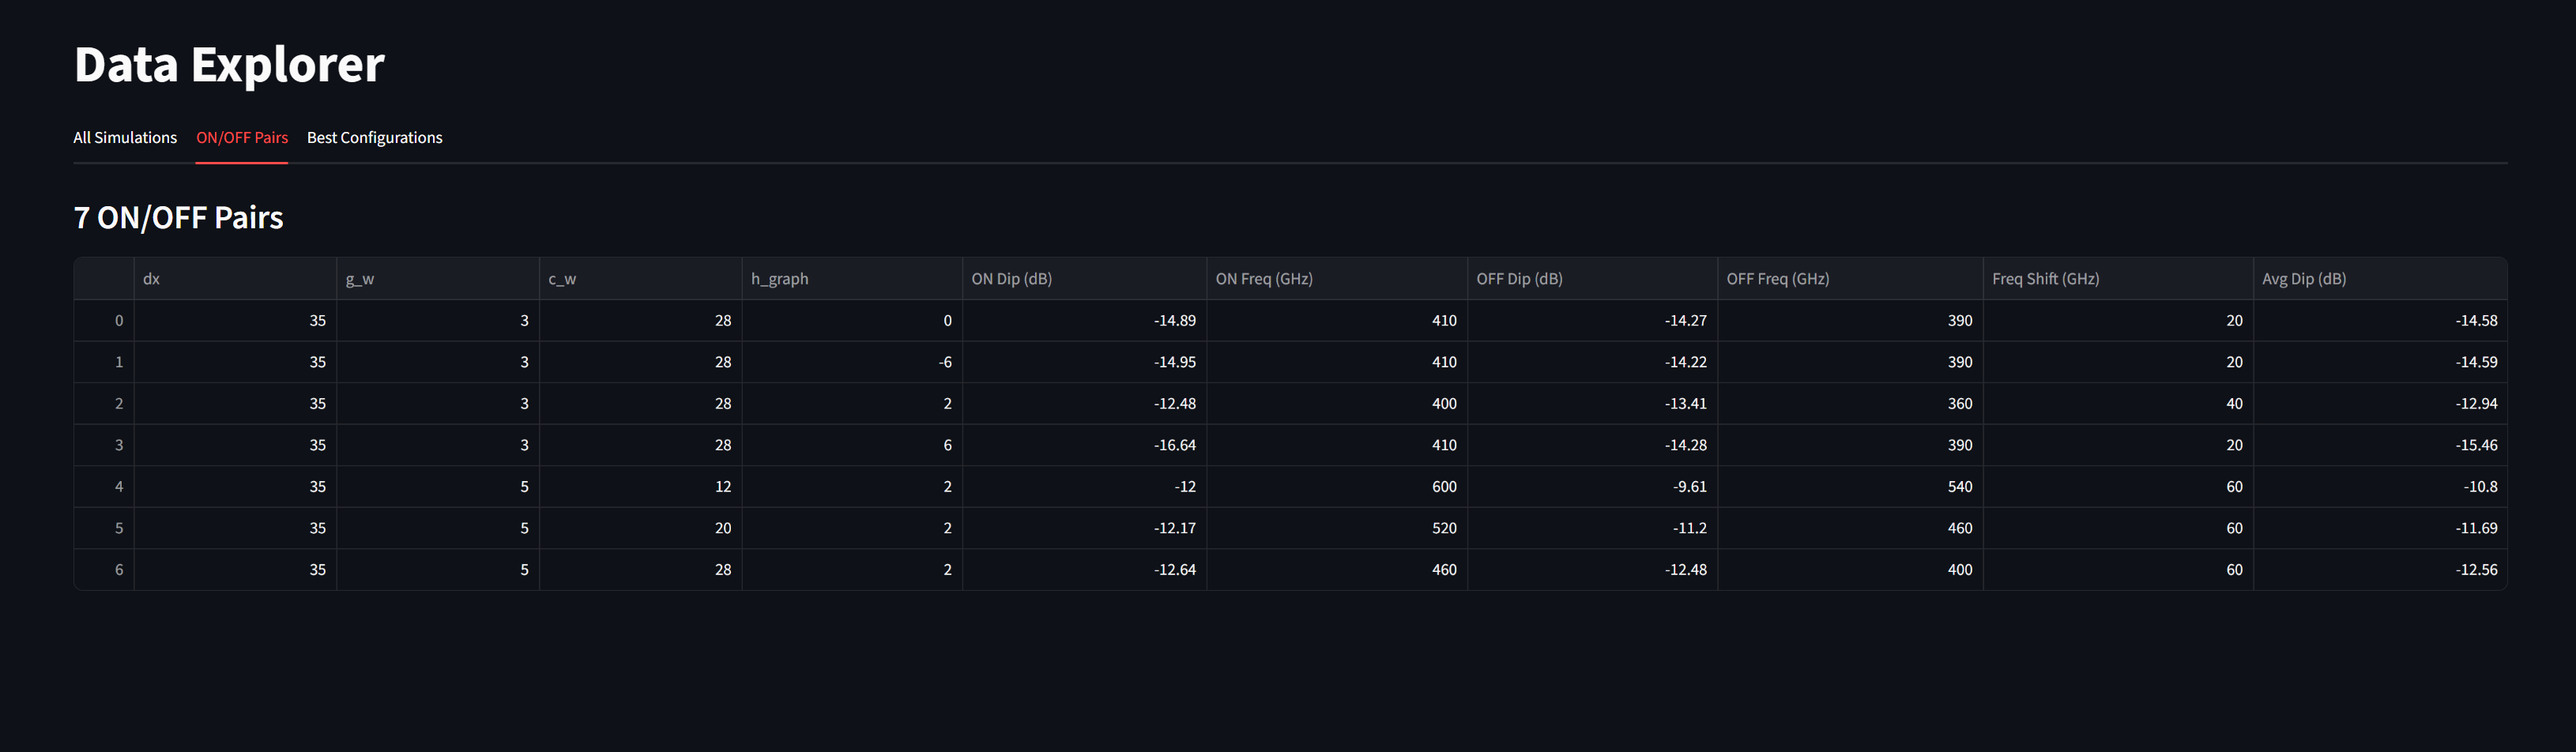
\includegraphics[width=0.9\textwidth]{dashboard_onoff_pairs.png}
    \caption{ON/OFF pairs page showing the 7 paired simulations with their frequency shifts and dip depth differences.}
    \label{fig:app_onoff_pairs}
\end{figure}

\begin{figure}[H]
    \centering
    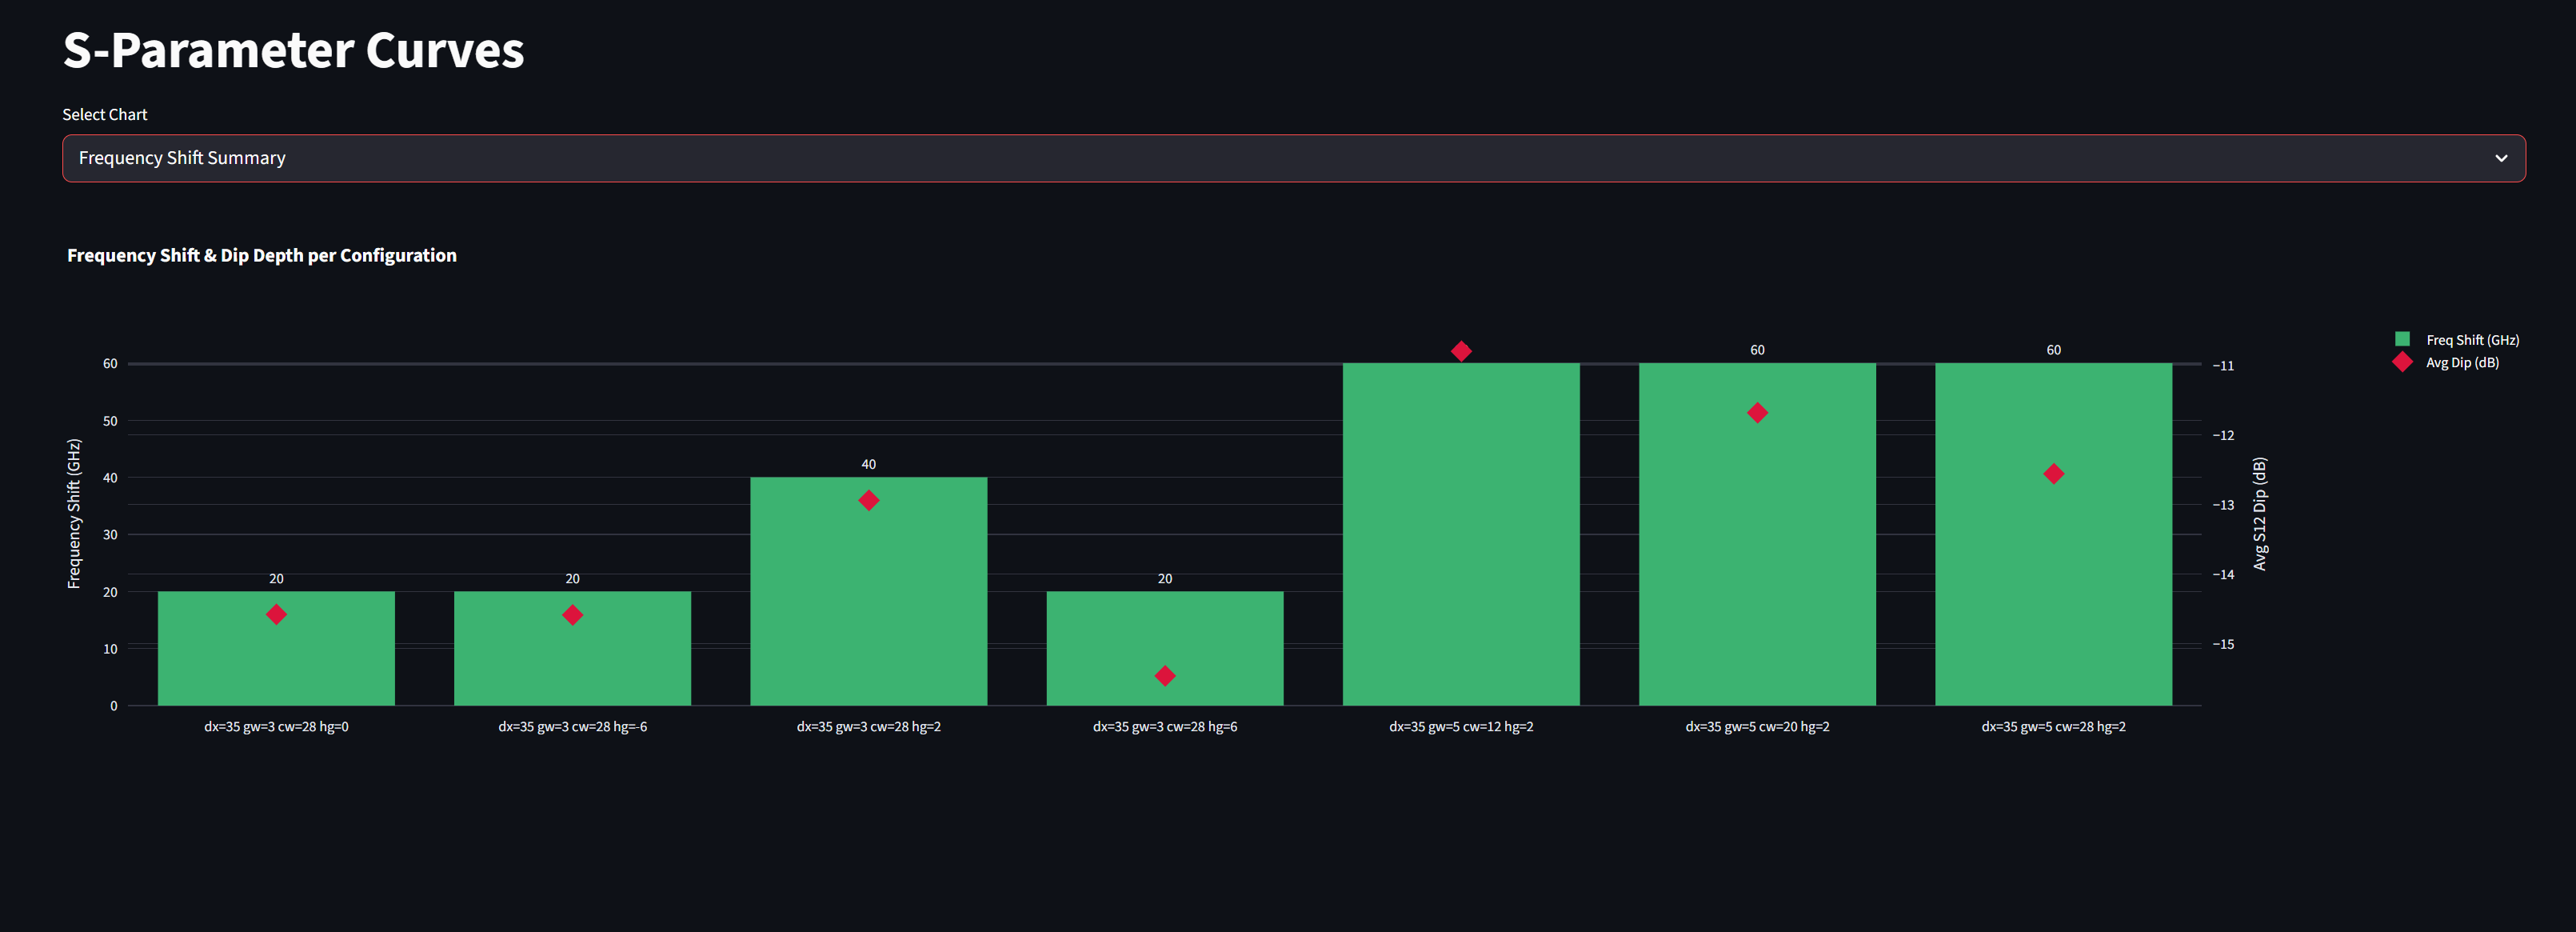
\includegraphics[width=0.9\textwidth]{dashboard_freq_shift.png}
    \caption{Frequency shift bar chart showing the ON/OFF frequency difference for each paired simulation.}
    \label{fig:app_freq_shift}
\end{figure}

\chapter{Generative AI Declaration}
\label{app:genai}

In accordance with Queen Mary University of London's academic integrity policy, the following declaration is made regarding the use of generative artificial intelligence (AI) tools in the preparation of this project.

\section*{AI Tools Used}

\begin{itemize}[leftmargin=2cm]
    \item \textbf{Claude} (Anthropic) --- accessed via Claude Code CLI (command-line interface)
\end{itemize}

\section*{How AI Was Used}

Generative AI was used in the following specific capacities during this project:

\begin{enumerate}[leftmargin=2cm]
    \item \textbf{Code development assistance:} AI was used to assist with the development of the Python data pipeline (\texttt{data\_loader.py}), machine learning training framework (\texttt{ml\_model.py}), Streamlit dashboard (\texttt{streamlit\_app.py}), and visualisation scripts (\texttt{visualize.py}, \texttt{analyze.py}). This included assistance with code structure, debugging, and implementation of specific functions.

    \item \textbf{Report writing assistance:} AI was used to assist with drafting sections of this \LaTeX{} report, including structuring the document, formulating academic prose, and formatting tables, figures, and equations.

    \item \textbf{Diagram generation:} AI was used to generate Mermaid diagram code for the ML workflow pipeline and algorithm concept visualisations (Figures~\ref{fig:rf_concept}--\ref{fig:loo_cv}).
\end{enumerate}

\section*{Work Performed Independently by the Student}

The following aspects of the project were performed entirely by the student without AI assistance:

\begin{itemize}[leftmargin=2cm]
    \item All COMSOL Multiphysics electromagnetic simulations were configured, executed, and monitored manually by the student.
    \item All simulation data was collected, organised, and verified by the student.
    \item The selection of machine learning models (Random Forest, Gradient Boosting, Gaussian Process) and evaluation strategy (LOO~CV) was decided by the student based on dataset characteristics.
    \item All results were independently interpreted, validated against physical expectations, and critically analysed by the student.
    \item The overall project direction, research questions, and conclusions were formulated by the student in consultation with the supervisor.
\end{itemize}

\section*{Statement of Responsibility}

I confirm that all AI-generated content has been carefully reviewed, verified for accuracy, and revised where necessary. I take full responsibility for the accuracy, originality, and academic integrity of all work presented in this report. The use of AI tools was supplementary to, and did not replace, my own understanding and critical analysis of the subject matter.

\vspace{1cm}
\noindent\textbf{Signed:} Linah Salem Alrejaee \\
\textbf{Date:} March 2026

\end{document}
